%%% use twocolumn and 10pt options with the asme2ej format
\documentclass[twocolumn,cleanfoot,10pt]{asme2ej}
%\usepackage{epstopdf}
\usepackage{epsfig} %% for loading postscript figures
\usepackage{graphicx}
\usepackage{epstopdf}
\usepackage{float}
\usepackage{amsmath}
\usepackage{subcaption}
\usepackage{stfloats}
\usepackage{threeparttable}

\usepackage{array}
\usepackage{algorithmic}
\usepackage{algorithm}
\usepackage{multirow}
\usepackage{rotating}
\usepackage{mathrsfs}
\usepackage{color}
\usepackage[normalem]{ulem}
%\usepackage{multirow}
% for figures: caption label is italic, the caption text is bold / italic
\captionsetup[figure]{labelfont=bf,textfont=bf}
\captionsetup[table]{labelfont=bf,textfont=bf}


% \linespread{2}
%% The class has several options
%  onecolumn/twocolumn - format for one or two columns per page
%  10pt/11pt/12pt - use 10, 11, or 12 point font
%  oneside/twoside - format for oneside/twosided printing
%  final/draft - format for final/draft copy
%  cleanfoot - take out copyright info in footer leave page number
%  cleanhead - take out the conference banner on the title page
%  titlepage/notitlepage - put in titlepage or leave out titlepage
%  
%% The default is oneside, onecolumn, 10pt, final


\title{A lower limb exoskeleton recycling energy from knee and ankle joints to assist push-off}

%%% first author
\author{Yihua Chang
	\affiliation{
		State Key Laboratory of Tribology\\
		Tsinghua University\\
		Beijing, China, 100084\\
		Email: changyh16@mails.tsinghua.edu.cn
	}	
}

\author{Weixin Wang
    \affiliation{
	State Key Laboratory of Tribology\\
	Tsinghua University\\
	Beijing, China, 100084\\
    Email: weixinwang442@gmail.com
    }	
}

\author{Chenglong Fu\thanks{Corresponding author.}
    \affiliation{ 
    Department of Mechanical and Energy Engineering\\
	Southern University of Science and Technology\\
	Shenzhen, China, 518055\\
	Email:  fucl@sustech.edu.cn
    }
}



\begin{document}

\maketitle    

%%%%%%%%%%%%%%%%%%%%%%%%%%%%%%%%%%%%%%%%%%%%%%%%%%%%%%%%%%%%%%%%%%%%%%
\begin{abstract}
{\it This paper presents the design and preliminary evaluation of a quasi-passive lower limb exoskeleton that was designed to improve walking efficiency. During walking, lower limb joints perform both positive and negative work. The exoskeleton recycles the negative mechanical work performed by knee joint in late swing and ankle joint in mid-stance, to assist the ankle joint in late stance when a burst of positive power is needed. The exoskeleton consists of a torque spring as an energy storage element and two clutches at each end of the spring to control the timing of recycling and releasing energy in a gait cycle. The two clutches are actively controlled by two small servo motors with very low power consumption based on the plantar pressure. The novelty of this exoskeleton lies in the fact that it makes the extra kinetic energy dissipated at knee joint reusable by transferring it to ankle joint to assist positive power generation during push-off for the first time. Eight male subjects walked with the exoskeleton engaged (EXO\_ON), disengaged (EXO\_OFF) and without the exoskeleton (NO\_EXO). Inverse dynamics analysis demonstrated that, the total biological negative knee work during the late swing phase reduced by of 15.9\% and the total biological ankle positive work during stance phase reduced by 29.7\% when comparing the EXO\_ON condition to the EXO\_OFF condition. The results proved the effectiveness of the exoskeleton at joint level.
	
Keywords: ankle exoskeleton; lightweight motor; power amplification}


\end{abstract}

%%%%%%%%%%%%%%%%%%%%%%%%%%%%%%%%%%%%%%%%%%%%%%%%%%%%%%%%%%%%%%%%%%%%%%


%%%%%%%%%%%%%%%%%%%%%%%%%%%%%%%%%%%%%%%%%%%%%%%%%%%%%%%%
%%%                                     
%%%  1. Introduction                    
%%%                                     
%%%%%%%%%%%%%%%%%%%%%%%%%%%%%%%%%%%%%%%%%%%%%%%%%%%%%%%%
\section{Introduction}       
\label{sec:intro}

Humans consume more energy when walking than any other activity in daily life. For a long time, researchers have been attempting to develop lower limb exoskeletons to enhance or assist human locomotion. However, the excessive requirement of power at lower limb joints during walking leads to undesirable size and weight of actuators\cite{RN1}. For instance, the peak value of ankle joint power during late stance plantar flexion is about 270W for a 70kg person\cite{RN2}. Therefore, designers have to make a tradeoff between the assisting capability and portability. To circumvent this dilemma, passive/quasi-passive exoskeletons were proposed\cite{RN3}. These exoskeletons do not directly provide external energy to human. \sout{They use some smart mechanical structures to provide energy by means of utilizing power from other joints, ground reactions or other synergistic action and make locomotion more energetically efficient.} \textcolor{red}{Instead, they use some smart mechanical structures to recycle the dissipated energy during decelerating segments in walking, and supply this recycled energy when positive power is required.}

The idea of these passive exoskeletons is that they use passive elements, mostly dampers or springs, instead of powerful actuators to apply external torques at the lower limb joints. The damper is a pure energy dissipative element to dissipate excessive kinetic energy during locomotion, which would otherwise cost extra physiological energy\cite{negativework}. The exoskeleton built by Walsh \emph{et al.} uses a magnetorheological damper to help knee joint produce negative work during normal walking\cite{RN3}. The spring in theory does not produce or dissipate energy, but its ability to store and return energy makes it a good candidate to interact with human limbs. 

Energy storage and return is also a high energetically efficient mechanism in human walking. The muscle-tendon unit serves as an energy storage element during walking \cite{RN16}\cite{pays}. By replacing tendons with springs, mechanical structures can relax the attached muscles which should otherwise produce forces to provide an anchor to one end of the tendon. Exoskeletons described in \cite{RN3}\cite{RN4}\cite{RN5} have springs spanning hip joint and ankle joint or only ankle joint to work as alternative mechanism for energy storage and return. In addition, springs are also used to shape the biological leg stiffness during stance phase in running, or in other words, decrease the large load exerted at joints after heel strike \cite{RN6,RN7,RN8}.

Among these exoskeletons, using external moment to assist late stance ankle plantar flexion is well proved to benefit to human by many other active exoskeletons\cite{RN5,RN9,RN10,RN11,RN12}. The exoskeleton built by Collins \emph{et al.}\cite{RN5} used a spring to assist Achilles tendon to store energy in dorsiflexion during stance phase and then release the energy to assist the following ankle plantar flexion, which successfully reduces the metabolic expenditure during walking. \sout{However, the optimal peak power of this passive ankle exoskeleton \cite{RN5} is only 0.3Nm/kg, which did not reach the theoretical optimal power effect\cite{zhang2017human}.}
\textcolor{red}{In another work \cite{zhang2017human}, the authors even further reduced walking metabolic expenditure by applying an optimized assistive torque at ankle, which appeared higher than the torque supplied by the quasi-passive exoskeleton in \cite{RN5}. This may suggest in stead of only recycling passive work from ankle dorsiflexion in stance, it could be beneficial to have another energy source for ankle assistance.}

From another perspective, knee joints absorb energy in most of a gait cycle\cite{RN2}, therefore we can also use a spring instead of a damper in\cite{RN3}, to apply resistive torques at knee joints and recycle the negative work at the same time. This part of energy can be treated as ‘external’ energy input at ankle joints, which means it may be beneficial to human if the energy from knee joints can be recycled to assist ankle joint in late stance plantar flexion. This concept has also been mentioned in some other studies\cite{RN3} \cite{RN12}, but no such actual devices have been reported to the best of the authors' knowledge.

In this paper, we present a quasi-passive lower limb exoskeleton which is able to recycle energy from both the extension movement of knee joint in late swing phase and dorsiflexion of ankle joint in mid-stance phase to assist ankle plantar flexion in late stance phase. The exoskeleton consists of a torque spring to store energy and two clutches to control the timing of energy recycling and releasing based on foot contact information. In order to evaluate the effectiveness of the exoskeleton, the power of exoskeleton was measured to estimate the amount of energy recycled and released; inverse dynamics analysis was also performed to evaluate the benefits and side-effects to human during walking.

The rest of this paper is organized as follows. In section \ref{sec:design}, the design of the proposed exoskeleton is introduced. Then the experiment setting and results are presented in section \ref{sec:experiment}. Finally, conclusion and future work are given in section \ref{sec:discussion}.


%%%%%%%%%%%%%%%%%%%%%%%%%%%%%%%%%%%%%%%%%%%%%%%%%%%%%%%%
%%%                                     
%%%  2. Design                 
%%%                                     
%%%%%%%%%%%%%%%%%%%%%%%%%%%%%%%%%%%%%%%%%%%%%%%%%%%%%%%%
\section{Design of Exoskeleton}
\label{sec:design}

\subsection{Design Objective}
\label{subsec:Biomechanics}

	Lower limb joints (mainly hip, knee and ankle) perform both positive work and negative work during each stride cycle of human walking, as shown in Figure \ref{fig:work}. The stance leg transports the center of mass of human body along an arched path, usually compared to an inverted pendulum\cite{RN13}. Before toe off, there is an intensive burst of energy generated at the ankle (red \textcolor{red}{solid} area, 40-60\% Stride, Figure \ref{fig:work}). This part of energy is consumed to redirect the downward velocity of the center of mass to the upward direction and initiate the next step as part of the step-to-step transition \cite{RN14}. This process is referred to as push-off, in which the energy dissipation in the collision between the opposite leg and ground is compensated by the energy generated at ankle, which costs nearly 45\% of the metabolic energy expenditure of human walking\cite{RN15}.

\begin{figure}[b]
	\centering
	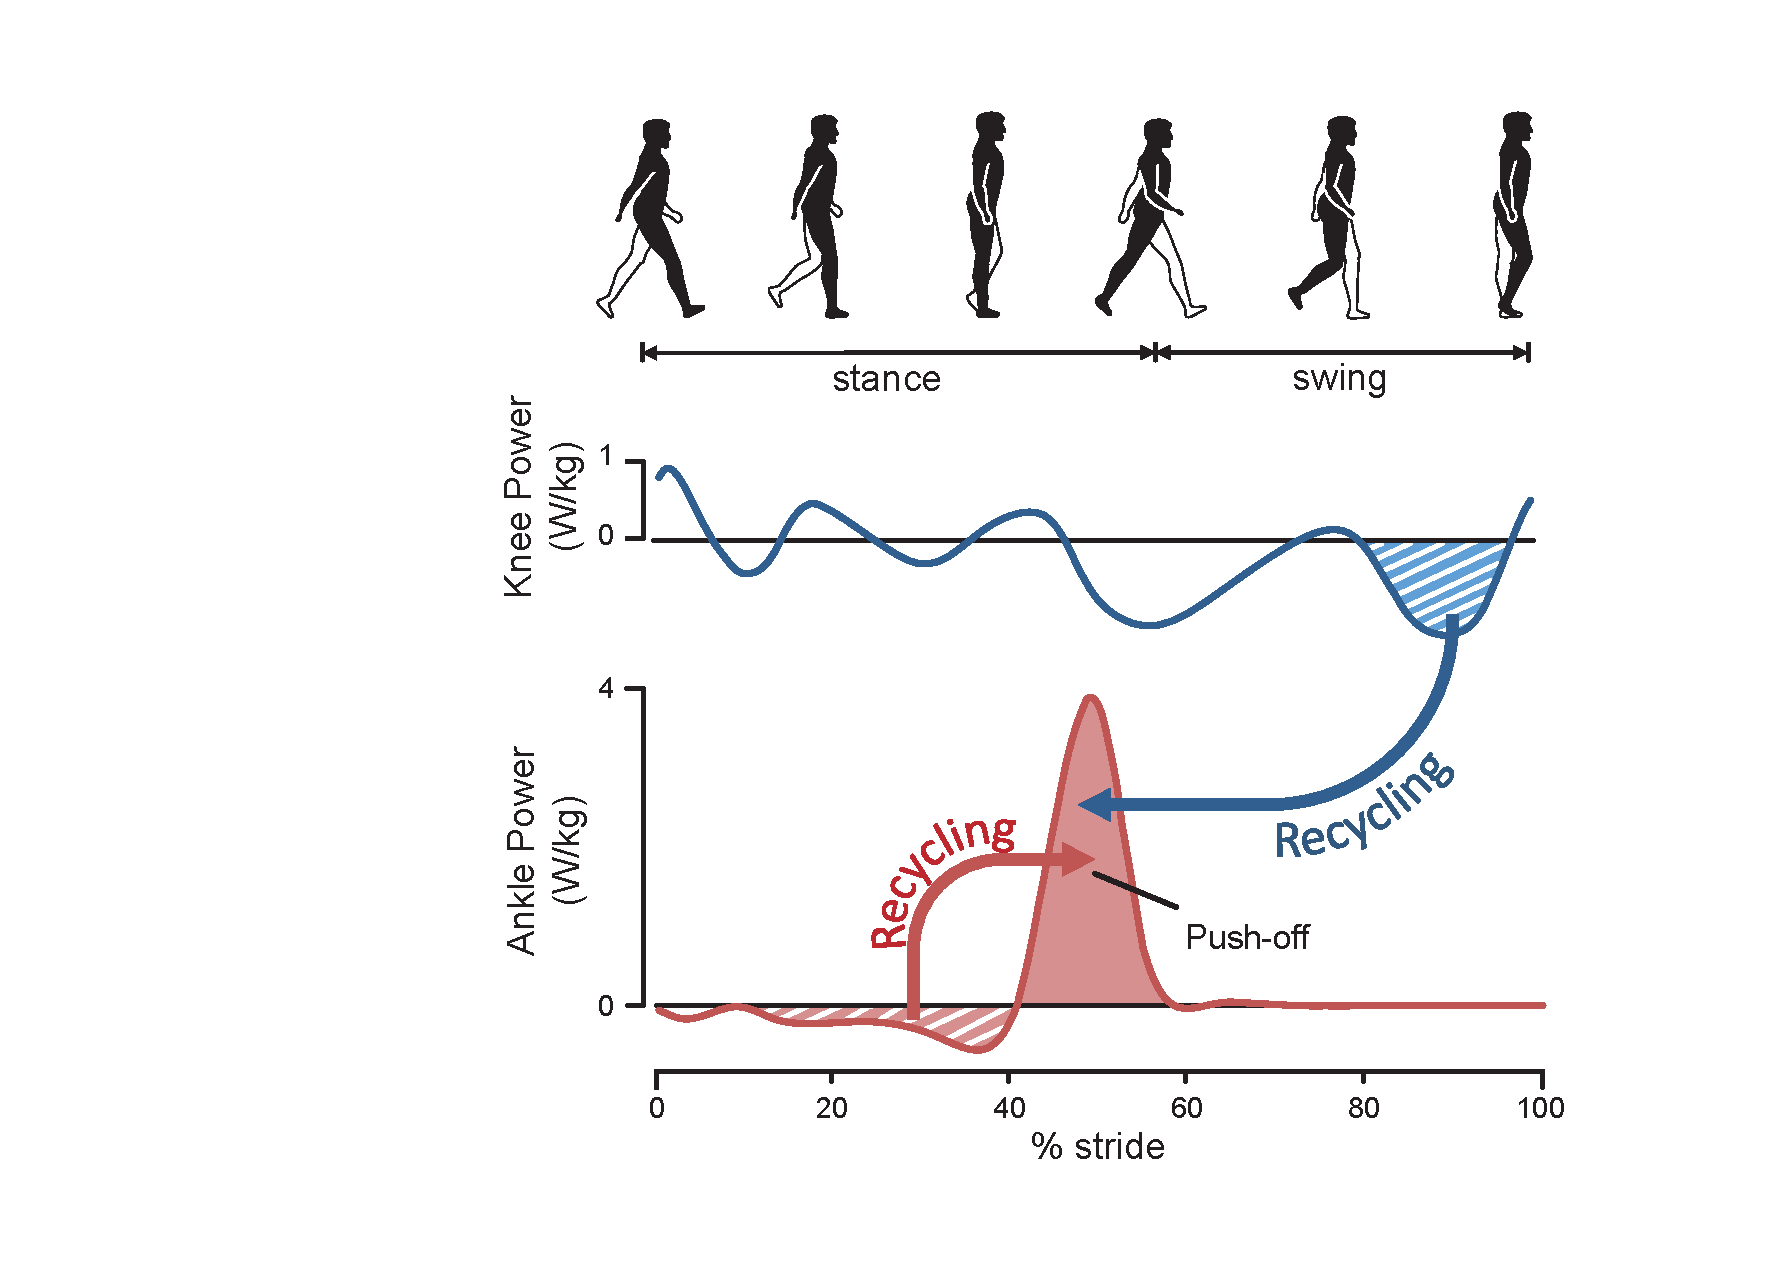
\includegraphics[width=0.45\textwidth]{Figure1.eps}
	\caption{Joint power of human walking and concept of energy recycling. A typical work rate of knee and ankle joint over a walking stride is shown (adapted from \cite{RN2}). The negative work performed by knee in terminal swing (blue hatched area) and ankle in mid-stance (red hatched area) is a possible source of energy for push-off (red \textcolor{red}{solid} area).}
	\label{fig:work}   
\end{figure}

\sout{The main challenge in designing a passive exoskeleton is that, even if we know how to assist human, it is still very difficult to recycle negative work from human without too many side-effects.} \textcolor{red}{Even though we know the best place and time to supply energy, designing a passive exoskeleton is still challenging since it needs to recycle energy from human without adding hindering forces or moments.} Measurements in vivo have suggested that considerable negative work performed by ankle dorsiflexion was stored in the Achilles tendon and used for the following push-off\cite{RN16}. In this process, the mechanical behavior of the Achilles tendon resembles a spring which is stretched during dorsiflexion to store energy and recoils during plantar flexion to release energy. \sout{Nonetheless, plantar flexors (gastrocnemius and soleus) should contract isometrically to provide an anchor for Achilles tendon when it is stretched. For the isometric contraction metabolic energy is consumed though no mechanical energy is produced by these muscles\cite{RN17}. Thus, we can assume that it is feasible to obtain the negative work from ankle in its dorsiflexion motion during stance (red hatched area, 15-40\% Stride, Figure \ref{fig:work}) to replace the function of Achilles tendon and relax ankle plantar flexors.} \textcolor{red}{Though no mechanical energy input is needed, the plantar-flexors (gastrocnemius and soleus) need to provide a force which makes the proximal end of Achilles tendon fixed in order to store energy. This force is achieved through muscle isometric contraction, which requires metabolic energy expenditure though no mechanical energy is produced \cite{RN17}. Thus, in this paper we propose it is beneficial to recycle negative work from ankle in its dorsiflexion motion during stance (red hatched area, 15-40\% Stride, Figure \ref{fig:work}) with a physical spring and fixation of its proximal end, so that plantar-flexors are freed from exerting the force.}

In terminal swing phase, the knee joint performs a large amount of negative work when it extends (blue hatched area, 80-100\% Stride, Figure \ref{fig:work}). During this period, thigh and shank can be modelled as a jointed double-pendulum pinned at knee joint\cite{RN2}. When knee extends, the lower segment (shank) of the jointed pendulum is returning to its neutral position, being accelerated by gravity. To prevent hyper-extension, knee should perform negative work to decelerate the shank and this process is accomplished by knee flexors (mainly hamstrings). Recycling the negative work performed by knee is similar to a regenerative braking decelerating a hybrid car, where the harvested energy can be reused in other applications. A device assisting knee in decelerating in principle can bring benefits to human and obtain energy at the same time. An energy harvester using this part of energy to generate electricity demonstrated very high efficiency, which generates every watt of electricity with only 0.7 watt of metabolic cost increased\cite{RN18}. For this reason, an exoskeleton also holds considerable promise to obtain energy from knee extension during swing to assist ankle push-off.

\subsection{Mechanical Design}

\begin{figure}[b]
	\centering
	\includegraphics[width=8.5cm]{Figure2.eps}
	\caption{Mechanical design of quasi-passive exoskeleton. (a) schematic of exoskeleton highlighting key components; (b) quasi-passive exoskeletons worn on a participant}
	\label{fig:model}   
\end{figure}

There are several design characteristics that the exoskeleton may use to achieve design purpose. Firstly, as depicted in subsection \ref{subsec:Biomechanics}, this exoskeleton is designed to assist ankle plantar flexion during push-off using the negative work recycled from both knee joint in late swing and ankle joint in mid-stance of human walking. Secondly, because of the energy recycled from knee and ankle joints will be released approximately half of a gait cycle afterwards (from late swing to the next late stance), the exoskeleton should also be able to store the energy for a specific amount of time. Thirdly, during the other parts of the gait cycle when the exoskeleton is not working functionally, it should not hinder the natural movements of lower limb. \sout{Finally, the exoskeleton should be lightweight and comfortable enough to minimize its side-effects.} \textcolor{red}{Finally, the exoskeleton should be lightweight and comfortable enough to mitigate the effects of added mass and extra kinematic constraints imposed by the structures.}

As shown in Figure \ref{fig:model}(a), the main idea of our device is to use two clutch to control the recycle and release of energy in a torque spring. Figure \ref{fig:model}(b) shows the quasi-passive exoskeleton worn on a healthy subject. The exoskeleton consists of a rigid ankle brace including the shank part and the ankle part, a torque spring and two motor controlled clutches which are integrated into a clutch-spring unit, compression baselayer pants, a pressure insole and electronic control system. The torque spring is used to store the recycled mechanical energy from knee joint and ankle joint. Two ends of the torque spring are fixed to two rotatory clutches, which are used to control the timing of recycling and releasing energy. The clutch-spring unit is fixed to the shank part of ankle brace. Two ropes are connected in series with the clutch-spring unit and span the knee joint (knee rope) and ankle joint (ankle rope) to \sout{track the joint angle and }exert external moment on the joints. 

When the exoskeleton works functionally, the two ropes exert resistive moment to the joints during energy recycling and assistive moment during energy releasing. The lower end of the ankle rope is fixed to the foot part of the ankle brace. Since knee joint rotates with a larger angle in swing extension than ankle joint does in late stance plantar flexion, the moment arm at ankle should be large enough to coordinate the travelling distance between the knee and ankle. For this reason, a aluminium alloy bar is extended posteriorly from the foot part of the ankle brace to provide a larger moment arm. 

\begin{figure}[b]
	\centering
	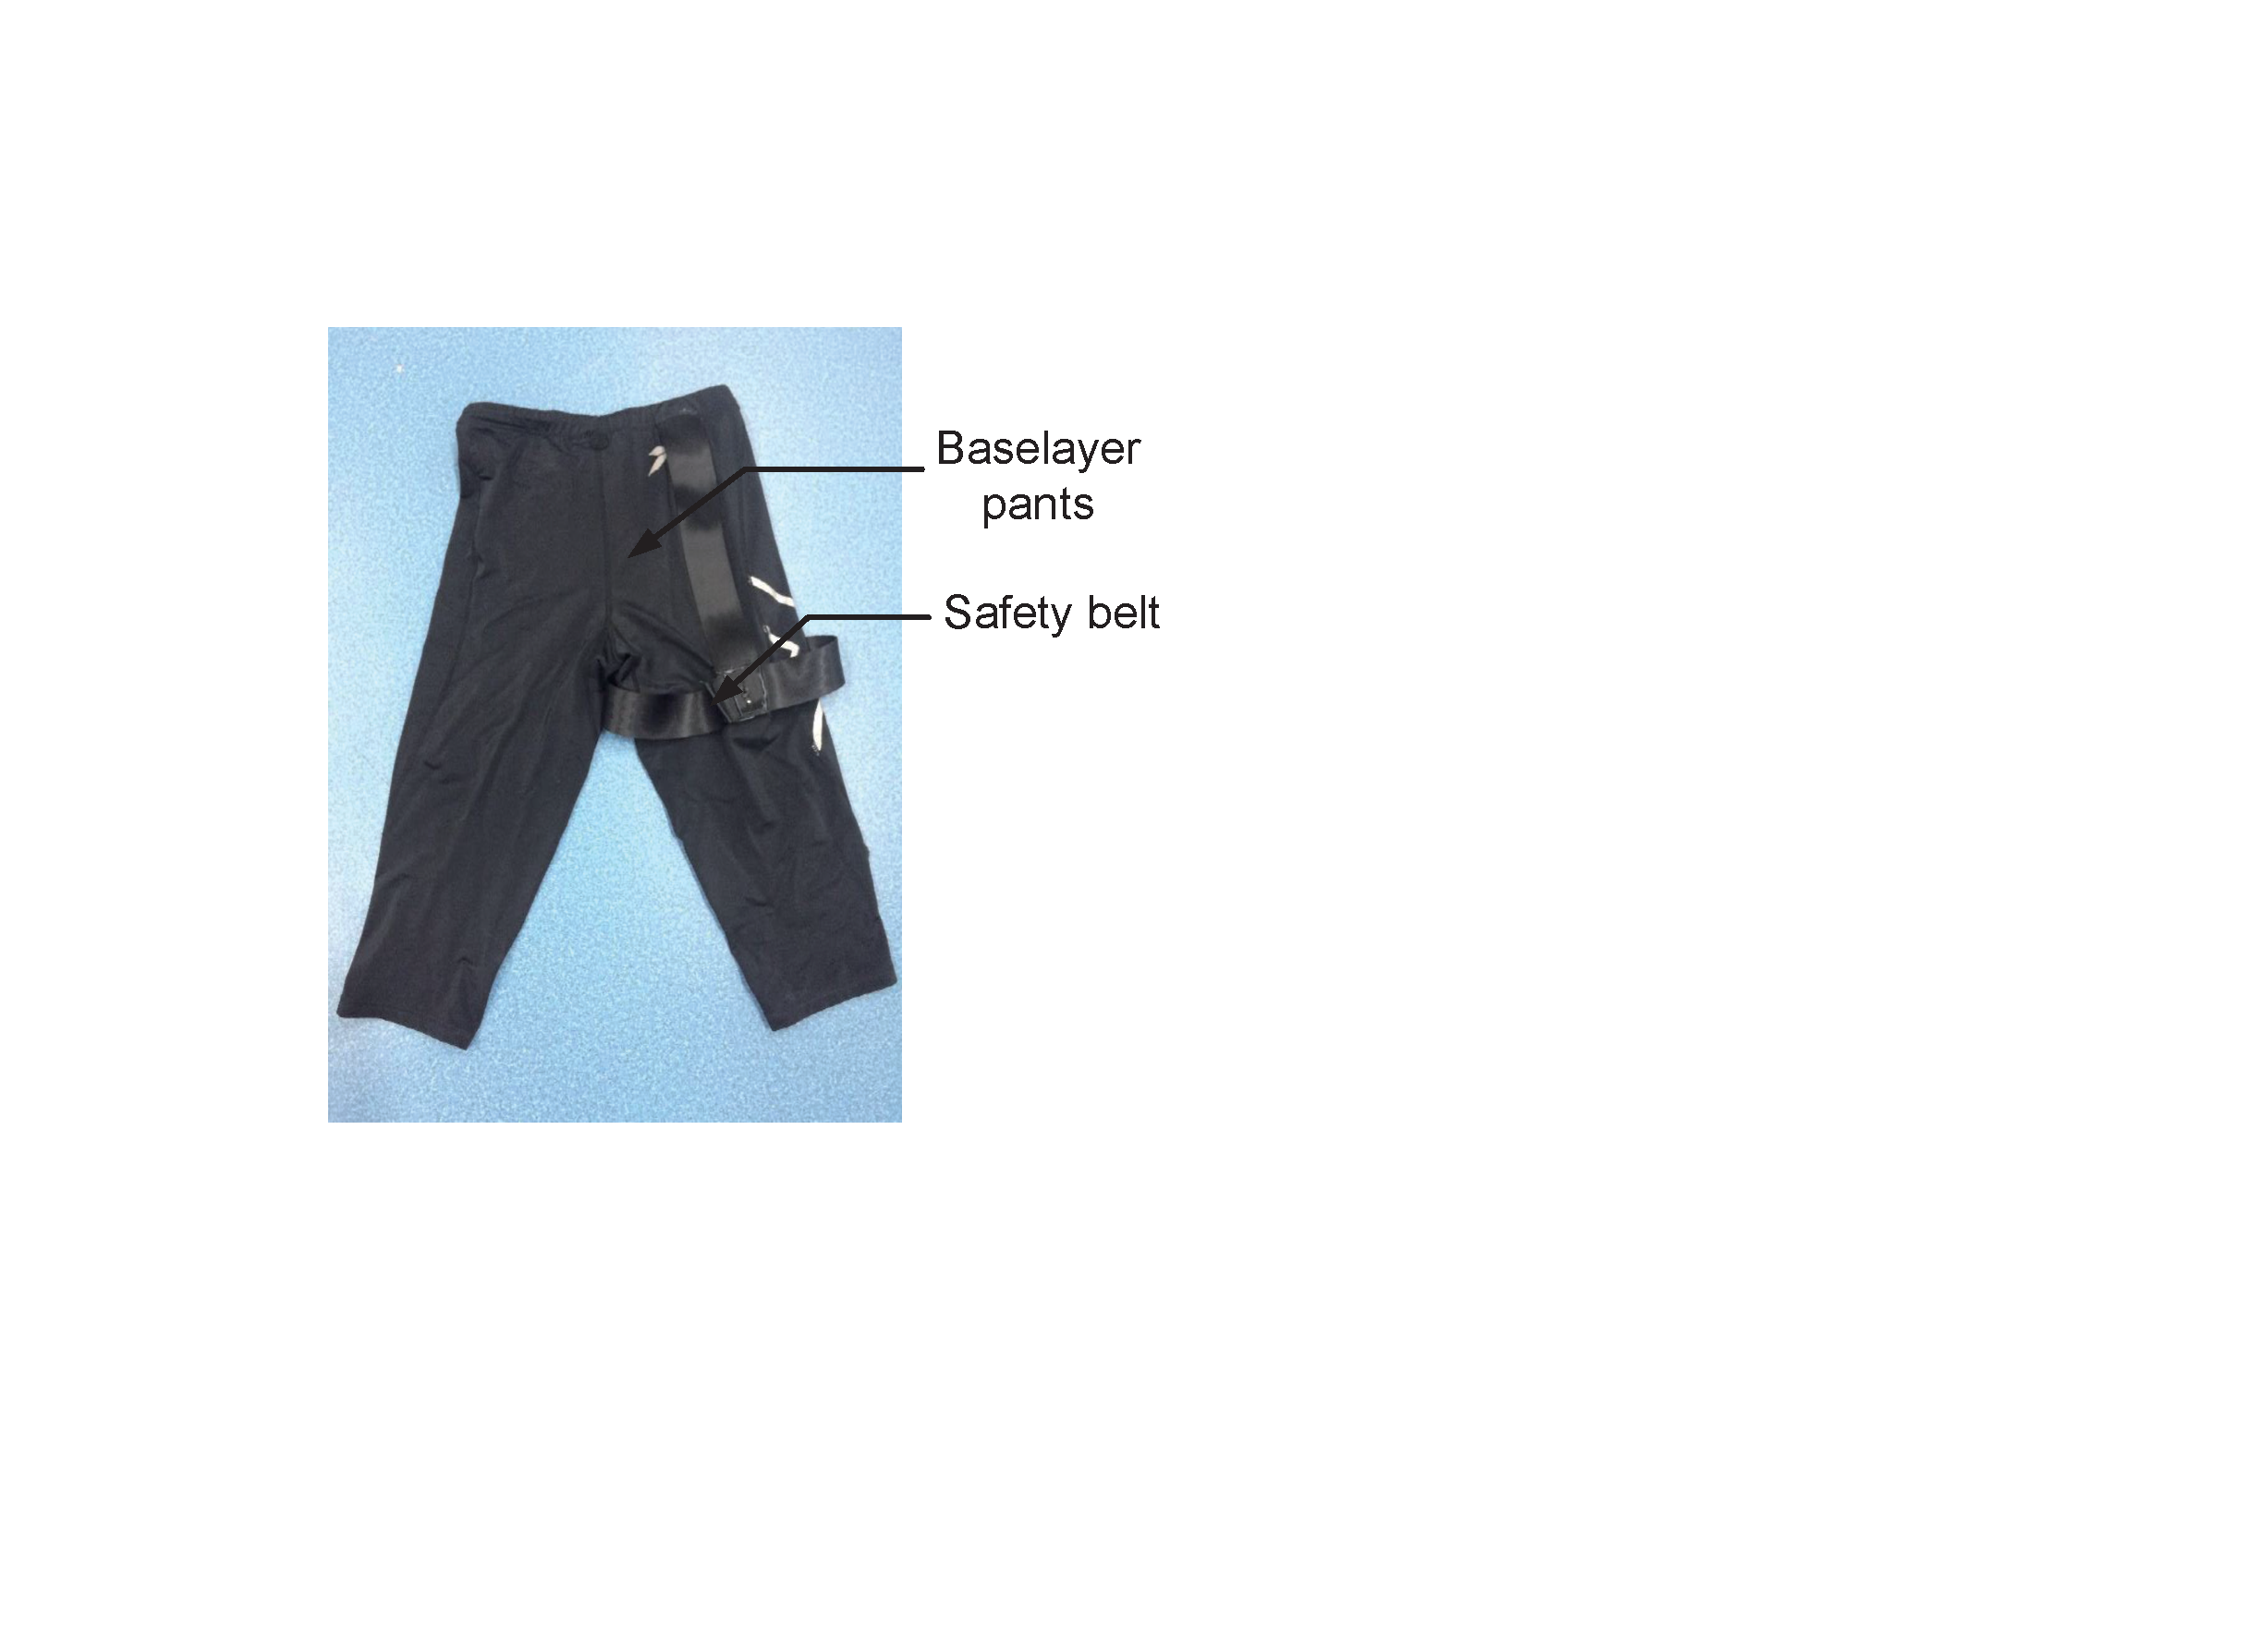
\includegraphics[width=8cm]{Figure3.eps}
	\caption{The thigh part: baselayer pants with seat belts sewn on.}
	\label{fig:pants}   
\end{figure}

Also, in principle, the knee rope should be rigidly fixed to the thigh. However, because human’s thigh tapers distally, the fixed point tends to slide off when a downwards force is exerted by the rope. However, the rigid hip brace may result in unacceptable weight. Therefore, inspired by the soft exo-suit developed by \cite{RN20}, we came up with an alternative solution, which uses baselayer pants to provide an elastic connection to the waist, as shown in Figure \ref{fig:pants}. In order to minimize the sliding between the pants and the thigh, non-deformable safety belts are sewed into the pants along the path through which the downwards force passes to the waist.

\begin{figure}[t]
	\centering
	\includegraphics[width=8.5cm]{Figure4.eps}
	\caption{Overview of the clutch-spring unit. (a)3D model highlighting key components; (b) exploded view}
	\label{fig:clutch}   
\end{figure}

The clutch-spring unit is the key part of the exoskeleton, which serves to recycle and release energy at specific durations in a gait cycle. The 3D model and exploded view of the clutch-spring unit are shown in Figure \ref{fig:clutch}. Instead of using an ordinary extension or compression spring, a torque spring is chosen as the energy storage element so that the two clutches at each end of the spring can be encapsulated with the spring together and assembled into a compact unit, which would not lead to a waste of space and extra weight. 

The design of the clutches is based on traditional ratchet, which is inspired by\cite{RN19}. The position of the pawl is actively controlled through gears by a small servo motor (DS215MG, KST Digital Technology, Guangdong, China) embedded in the shaft of the clutch-spring unit. The maximum output torque of the motor is 0.036 Nm. When the motor disengages the pawl, the ratchet wheel can rotate freely in both directions; when the motor engages the pawl, the ratchet wheel can only rotate in one direction. The motor is rigidly connected to the pawl in the disengaging direction and elastically connected in the engaging direction. The return elasticity of the pawl is realized by two small ratchet springs assembled between the motor shaft and the gear to push the pawl back when the ratchet wheel rotates in the allowable direction and potentially disengage the pawl.

There is a groove outside the ratchet wheel and can also serve as a pulley to hold the ropes. Each end of the torque spring is rigidly attached to the two ratchet wheels by screws and rope clamps. When the ratchets are engaged, the direction that releases the spring is prohibited, which means the elastic energy of the spring is locked into the clutch-spring unit when both clutches are locked and no force in the torque spring pass to the ropes. The shaft holding the two ratchets serves as the base frame of the spring-clutch unit and is rigidly fixed to the shank part of the ankle brace. Voids are also designed into the shaft to decrease its weight.

The total mass of the device is 832 g, with 623g worn on the shank and 209 g worn on the foot. A list of major components, model, material, mass and location is shown in
Table 1.  

%%%%%%%%%%%%%%% begin table   %%%%%%%%%%%%%%%%%%%%%%%%%%

\begin{table}[t]
	\caption{Exoskeleton component distribution}
	\begin{center}
		\label{tab:hardware}
		\begin{tabular}{c c c c}	
			\hline
			\textbf{Component} & \textbf{Model/Material} & \textbf{Mass} & \textbf{Location} \\
			\hline
			Servo motor & DS215MG & 19 g$\times$2 & Shank\\
			Battery & Lithium & 48 g & Foot\\
			Controller & Arduino nano & 21 g & Foot\\
			Clutch-spring & Aluminium alloy & 442 g & Shank\\
			Shank brace & Carbon fibre & 143g & Shank\\
			Foot brace & Carbon fibre & 110 g & Foot\\
			Supports & Aluminium alloy & 30g & Foot\\			
			\hline 
			\textbf{Shank part} & & \textbf{623 g} & \textbf{Shank}\\
			\textbf{Foot part} & & \textbf{209 g} & \textbf{Foot}\\
			\hline
			\textbf{Total} & & \textbf{832 g} & \\
			\hline
			
		\end{tabular}
	\end{center}
\end{table}



%%%%%%%%%%%%%%%% end table %%%%%%%%%%%%%%%%%%% 
\subsection{Working process}
\label{subsec:Working process}

\begin{figure*}[tb]
	\centering
	\includegraphics[width=17cm]{workingprocess.eps}
	\caption{The working process of the exoskeleton in a gait cycle]. Top: elastic potential energy in spring; middle: heel and toe contact with the ground, knee clutch and ankle clutch status; bottom: schematic of quasi-passive exoskeleton working conditions. The blue arrows show the rotation directions of the clutches and the black arrows show the movement directions of the rope.}
	\label{fig:workprocess}   
\end{figure*}

The working process of the exoskeleton in a gait cycle is shown in Figure \ref{fig:workprocess}, where 0\% and 100\% corresponds to two successive heel strikes. The description below will begin with the swing phase, for the complete energy recycling cycle of the exoskeleton is start at this point. At the beginning of the swing phase(Figure \ref{fig:workprocess}(a)), the two clutches are unlocked. During late swing (Figure \ref{fig:workprocess}(b)), the knee joint extends from its maximum flexion angle to full extension. As a consequence, the knee rope stretches the torque spring to harvest energy and apply a flexion torque at knee joint to assist hamstrings in decelerating the shank. The ankle clutch is locked before the knee joint starts extension in order to decouple the ankle joint so that the force in the spring can be exerted on the clutch instead of the ankle rope. Before the knee joint is fully extended, the knee clutch is locked to store the harvested energy.

In early stance (Figure \ref{fig:workprocess}(c)), the ankle joint naturally achieves foot flat through slight plantar flexion motion and the knee joint also undergoes slight flexion motion, both of which are in the direction that releases the energy in the torque spring. However, because the two clutches remain locked in this duration, both joints are decoupled from the torque spring. Therefore, the recycled energy in the torque spring is preserved and no force is passed to the ropes to cause adverse moments on the knee and ankle joint.

When the shank approaches the vertical position in mid-stance (Figure \ref{fig:workprocess}(d)), the torque spring begins to be stretched again by the ankle rope to recycle energy from ankle. The onset of recycling is determined by the original rope length, which can be adjusted to change the amount of energy recycled from ankle. It is important to unlock the ankle clutch during mid-stance when the ankle rope stretches the torque spring, because in this duration the pawl is unloaded and only a small torque from the motor is needed to disengage it. The knee clutch keeps locked throughout this process.

In late stance (Figure \ref{fig:workprocess}(e)), a burst of positive power is needed at the ankle joint to redirect the velocity of the center of mass of human. In this duration, the force in the spring is passed to the ankle rope and exerts a plantar flexion torque at ankle joint to perform positive mechanical work. As ankle plantar flexion progresses, the torque spring recoils and the previously recycled energy is finally released. The ankle clutch keeps unlocked throughout this process to allow force transmission between the torque spring and the ankle joint, while knee clutch keeps locked to decouple the knee joint from the spring at the same time.


After push-off, both ratchet wheels have rotated in the same direction for some angles compared with their initial positions. That means they should return to their initial positions to prepare for the next energy recycling cycle during initial swing (Figure \ref{fig:workprocess}(a)). In this process, because both pawls are disengaged, we can simplify the spring-clutch unit as a rigid body. That is, if one ratchet wheel returns to its initial position, the other returns automatically.

We use a return spring to accelerate the return process of the two ratchet wheels. The return spring is attached between the knee side ratchet wheel and the shaft fixed on the shank part of the ankle brace. So the return spring will drag the two ratchet wheels back to their initial position. An almost negligible side-effect is that when the torque spring is stretched in late swing, the return spring is also stretched, causing some extra energy wasted. However, the return spring can be much springier than the torque spring provided it can overcome friction forces to drag the ratchet wheels back. Therefore, the amount of energy wasted by the return spring should be negligible. 


\subsection{Control of the exoskeleton}


\begin{table*}[b]
	\centering
	\newcommand{\tabincell}[2]{\begin{tabular}{@{}#1@{}}#2\end{tabular}}
	\renewcommand{\arraystretch}{1.3}
	\caption{Allowable time interval and underfoot pressure criteria of clutch motion}
	\begin{center}
		\label{tab:control}
		\begin{tabular}{c c c c} 
			\hline
			\hline
			\multirow{2}{*}{\textbf{Clutch motion}} &  \multicolumn{2}{ c }{\textbf{Allowable time interval}} & \multirow{2}{*}{\shortstack{\textbf{Underfoot pressure criteria} \\ \textcolor{red}{(55 strides per minute)}}} \\ \cline{2-3}&\textbf{Start from} & \textbf{End before}\\
			\hline
			Ankle clutch locks&End of push-off&Beginning of knee extension&\tabincell{c}{0.1s after plantar \\ pressure disappears}\\
			Knee clutch locks&Beginning of knee extension&Heel strike&\tabincell{c}{0.2s after plantar\\ pressure disappears}\\
			Ankle clutch unlocks&Ankle in its neutral position&Beginning of push-off&\tabincell{c}{0.1s after forefoot\\ pressure appears}\\
			Knee clutch unlocks&End of push-off&End of push-off&\tabincell{c}{Right after plantar\\ pressure disappears}\\
			\hline
			\hline
		\end{tabular}
	\end{center}
\end{table*}


The control system of the exoskeleton(shown in Figure \ref{fig:control}) including an 800 mA$\cdot$h lithium battery, a small controller (Arduino NANO), two motors and a pressure insole. The supply voltage of Arduino NANO and the servo motor are 6V-8V and 4.5V-8.5V respectively. So the 8V lithium battery is used to power the measurement and control system. The supply voltage of the plantar pressure sensor uses the 5V output of the controller. 

Different from active exoskeleton, the control scheme of the quasi-passive exoskeleton is not to apply specific torques at lower joints by actuators, but to specify the timing to lock and unlock the two clutches. So it is reasonable to use the information of the foot pressure to control the timing of the clutch movements, as the most frequently referenced moment is push-off. The pressure insole is placed between the ankle brace and foot to detect the event of heel strike, toe off and mid-stance for timing control. Six force sensing resistor are sewed into an insole, which is placed between foot and the ankle brace. Four of them are placed under forefoot to detect toe off, while the rest two are placed under heel to detect heel strike. Because precise pressure measured by each force sensing resistor is not needed, the four sensors under forefoot and two under heel are electronically wired in parallel respectively. 

\begin{figure}[t]
	\centering
	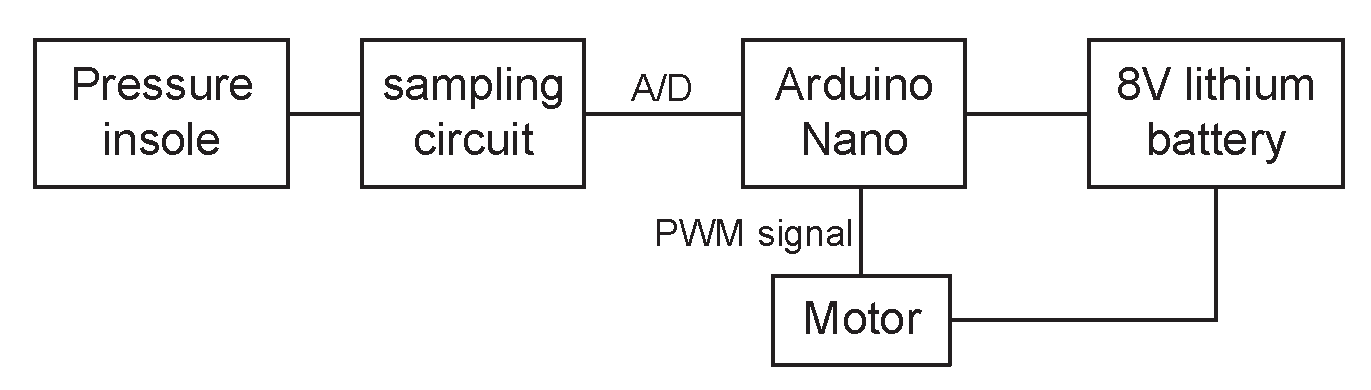
\includegraphics[width=8.5cm]{control.eps}
	\caption{The control system of the exoskeleton.}
	\label{fig:control}   
\end{figure}

Based on the discussions in the \ref{subsec:Working process}, locking and unlocking the ankle clutch as well as locking the knee clutch can be performed within some time intervals, whereas unlocking the knee clutch should be performed at a specific moment in a gait cycle. The detailed descriptions of the allowed time intervals to perform these clutch movements and the relationship between the movements of clutches and foot pressure signals are listed in Table \ref{tab:control}. \sout{Because there are no pressure throughout the swing phase, the movements of the clutches are controlled with predetermined time delay, according to the human normal walking speed 1.3m/s.} \textcolor{red}{In this current study, the timing of the clutches is per-determined according to the normal step frequency at 55 strides (full gait cycle) per minute (corresponding to around 1.3 m/s walking speed). More specifically, based on a typical gait cycle, the ankle and knee clutches should lock between 0s to 0.2s and between 0.2s to 0.4s after entering swing phase respectively, which motivates the choices of time delays listed in Table \ref{tab:control} after considering the delay in the mechanical system.}


\subsection{Parameter Design}

\label{sec:parameter design}


Human walking is highly optimized by evolution, improper torque applied at the joints may result in undesired results.  It has been found that even though the activity of plantar flexors assisted by an exoskeleton does not disappear totally, the activity of dorsiflexors begin to increase to counteract the effect of the exoskeleton, which leads to increased metabolic expenditure \cite{RN4}. Such muscle behavior is referred to as muscle co-contraction, which also happens between hamstrings and quadriceps, a pair of antagonistic muscle groups on the thigh. Hence, the best assisting strategy lies on the boundary at which the co-contraction is just about to happen \cite{RN22}. 

The boundary conditions of the negative power work that the exoskeleton recycles from the knee and ankle joints are determined by referencing to existing devices.
From the human subject experiment data in \cite{RN5,RN18}, they are roughly estimated as follows:
%While reducing the energy recycled in the ankle joint dorsiflexion to avoid muscle antagonism, the peak assisting power of the quasi-passive exoskeleton at late stance should be as large as possible. Referring to the knee energy harvester device designed by Donelan \emph{et al.}, the exoskeleton should be avoid to apply excessive moment to the knee joint at late swing phase. We set the boundary conditions for the exoskeleton as following (assuming the wearer weighs 65 kg):

(1) The peak negative power applied by the exoskeleton to the knee joint should be less 0.3 W/kg during knee extension in late stance, and the negative work recycled from the knee joint should not exceed 35\% of the biological negative work;

(2) The peak negative power applied by the exoskeleton to the ankle joint should be less than 0.2 W/kg during dorsiflexion in mid-stance, and the negative work recycled from the ankle joint should not exceed 10\% of the biological negative work.

\begin{figure}[t]
	\centering
	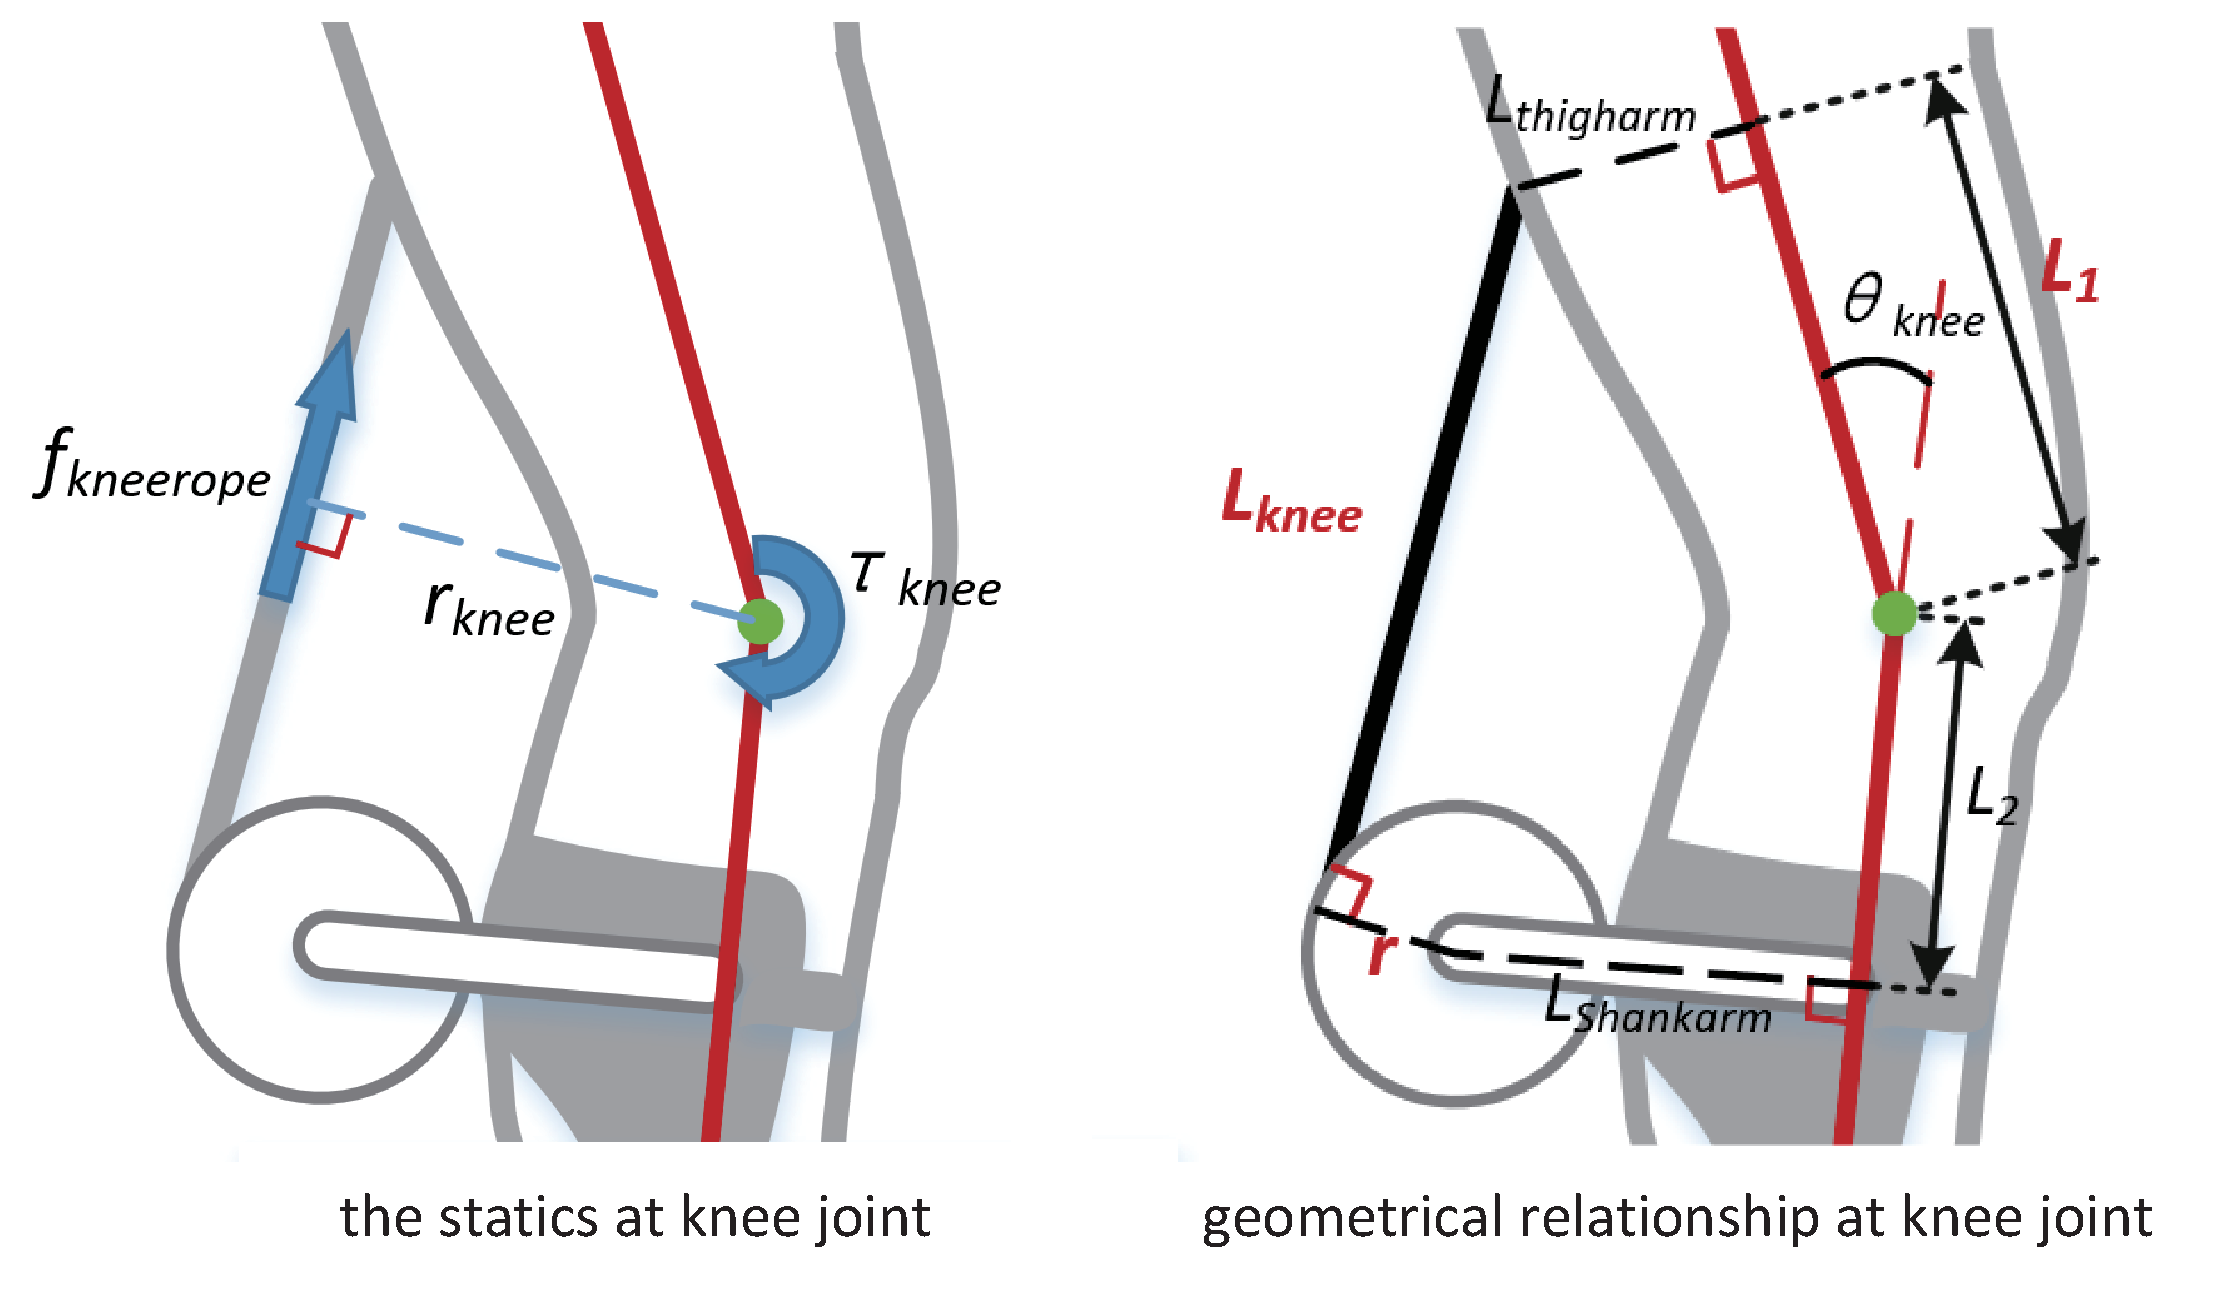
\includegraphics[width=8.5cm]{kneeparameters.eps}
	\caption{Statics and geometrical relationship between the exoskeleton and knee joint.}
	\label{fig:kneeparameters}
\end{figure}

\begin{figure}[t]
	\centering
	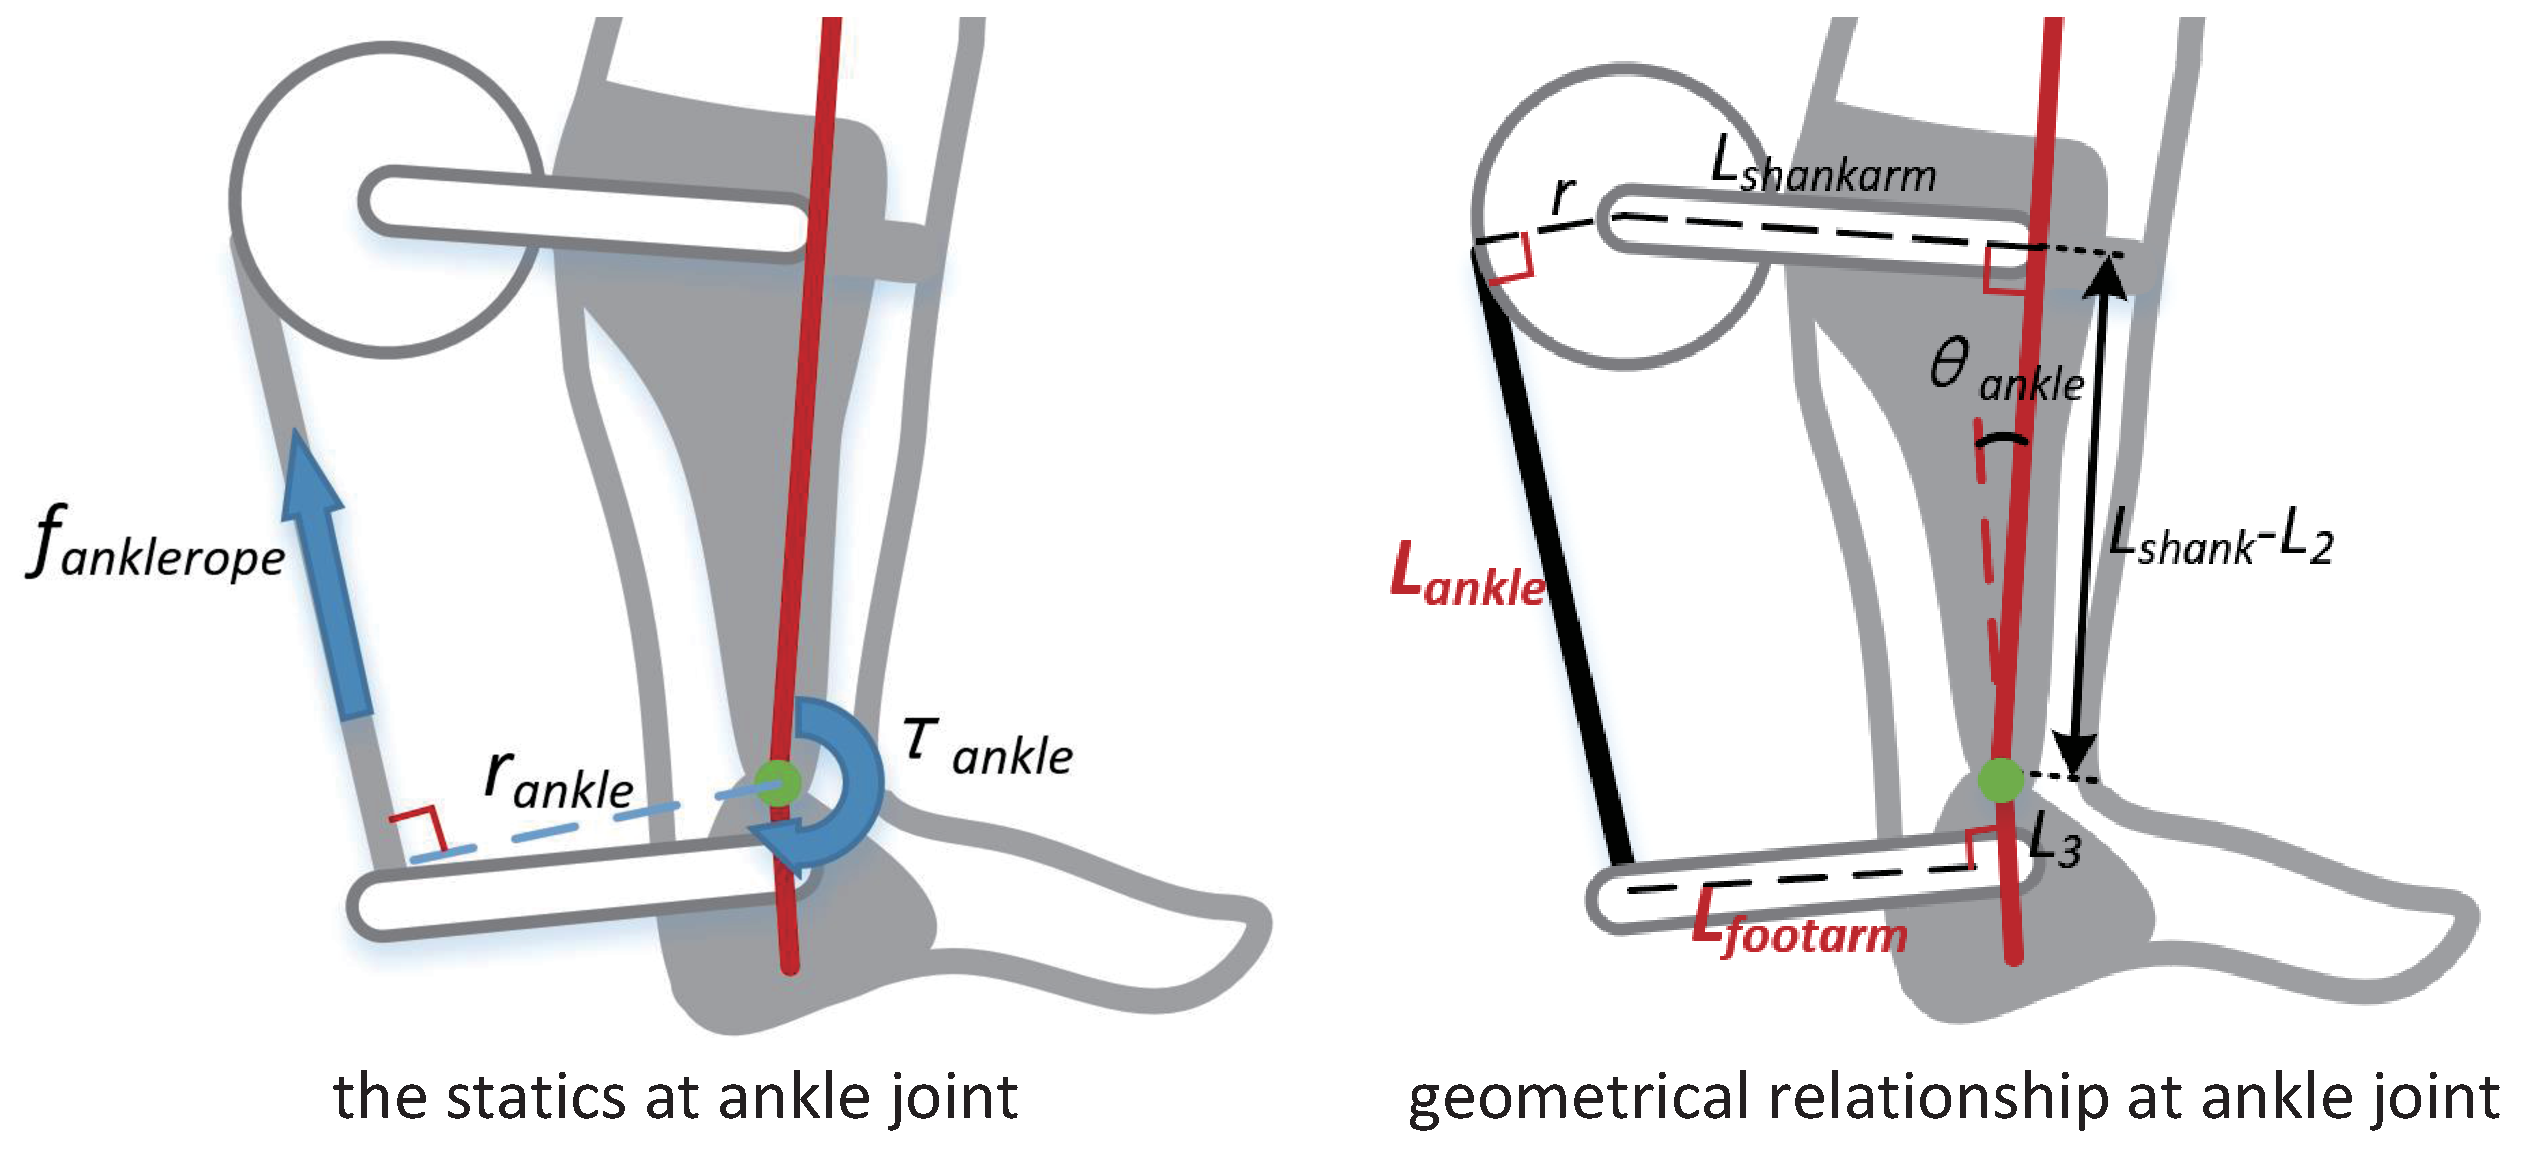
\includegraphics[width=8.5cm]{ankleparameters.eps}
	\caption{Statics and geometrical relationship between the exoskeleton and ankle joint.}
	\label{fig:ankleparameters}
\end{figure}

%The ratchet radius is $r$. The distance from the fixed point of the thigh to the center of the knee is $L_\textrm1$. The distance between the fixed point of the ankle brace to the center of the knee is $L_\textrm2$. The initial knee rope length is $L_\textrm{kneerope}^0$. The vertical distance from the center of the clutch-spring unit to the fixed point of the ankle brace is $L_\textrm{shankarm}$ (fixed to 10 cm). The distance between the thigh fixed point and the knee ratchet connection point can be calculated as $L_\textrm{knee}$ by the geometrical relationship. The length of the foot support bar is $L_\textrm{footarm}$.  The initial ankle rope length is $L_\textrm{anklerope}^0$. The distance between the foot fixed point and the ankle ratchet connection point can be calculated as $L_\textrm{ankle}$.

The tatics and geometrical relationships between the exoskeleton and joints are shown in Fig. \ref{fig:kneeparameters} and \ref{fig:ankleparameters}.
The forces in the two ropes spanning the knee and ankle joints while they are performing negative work are calculated as follows:
\begin{gather}
	f_\mathrm{kneerope} = \frac{k(L_\mathrm{kneerope}-L_\mathrm{kneerope}^0)}{r^2} \\
	f_\mathrm{anklerope} = \frac{k(L_\mathrm{anklerope}-L_\mathrm{anklerope}^0+\Delta L_\mathrm{kneerope})}{r^2},
\end{gather}
where $r$ is the ratchet radius, $k$ is the stiffness coefficient of the torsion spring, $L_\mathrm{kneerope}$, $L_\mathrm{anklerope}$ and $L_\mathrm{kneerope}^0$, $L_\mathrm{anklerope}^0$ are the length and initial length of the two ropes, and $\Delta L_\mathrm{kneerope}$ is the final length change of the knee rope after knee extension in late stance phase.

Then, using the notations in Fig. \ref{fig:kneeparameters} and \ref{fig:ankleparameters}, the negative power and work of the exoskeleton applied at the knee and ankle joints are
\begin{gather}
	P_\mathrm{knee} = r_\mathrm{knee}f_\mathrm{kneerope}\dot{\theta}_\mathrm{knee} \\
	P_\mathrm{ankle} = r_\mathrm{ankle}f_\mathrm{anklerope}\dot{\theta}_\mathrm{ankle} \\
	W_\mathrm{knee} = \frac{1}{2}k\Delta L_\mathrm{kneerope}^2 \\
	W_\mathrm{ankle} = \frac{1}{2}k(\Delta L_\mathrm{kneerope}+\Delta L_\mathrm{anklerope})^2 - W_\mathrm{knee}
\end{gather}
where $\dot{\theta}_\mathrm{knee}$, $\dot{\theta}_\mathrm{ankle}$ are the joint velocities, and $\Delta L_\mathrm{anklerope}$ is the final length change of the ankle rope after dorsiflexion in mid-stance.
From the normal values of the joint velocities and angles during walking at around 1.3 m/s, and the geometric relationships, we calculate the peak negative power and work of the exoskeleton as a function of the design parameters listed in Table \ref{tab:Exoskeleton parameters}.
Then based on the pre-determined upper bounds on the negative power and work, and assuming the wearer weighs 65 kg, we choose the design parameters accordingly.

%The energy that the exoskeleton recycled is:
%\begin{equation}
%W_\textrm{in}=W_\textrm{out}=\frac{1}{2}k(\phi(t_4))^2
%\end{equation}

%The torque and power are proportional to the stiffness coefficient of the spring. In the process of parameter selection, we first fix the stiffness coefficient of 1 Nm/rad. Then determine the shape of the assist power curve by adjusting the hardware parameters. The final selected parameter are shown in table \ref{tab:Exoskeleton parameters}.

\begin{table}[t]
	\caption{Exoskeleton parameters}
	\begin{center}
		\label{tab:Exoskeleton parameters}
		\begin{tabular}{c c}	
			\hline
			\textbf{Description } & \textbf{Value} \\
			\hline
			Spring stiffness & 1 Nm/rad\\
			Clutch inner radius & 29mm\\
			Clutch outer radius & 37.5mm\\
			Ratchet tooth angle & 30 degree\\
			$L_\textrm1$ & 110mm\\
			$L_\textrm2$ & 200mm\\
			$L_\textrm{anklerope}^0$ & 250mm\\
			$L_\textrm{shankarm}$  & 100mm\\
			$L_\textrm{anklerope}^0$ & 280mm\\
			$L_\textrm{footarm}$ & 200mm\\
			\hline
		\end{tabular}
	\end{center}
\end{table}

%%%%%%%%%%%%%%%% end table %%%%%%%%%%%%%%%%%%% 

The stiffness of the torsion spring can be used to change the maximum work that is able to be recycled by the exoskeleton without exaggerating the geometric parameters.
In this current prototype, the stiffness is chosen as 1 Nm/rad, which results in some appropriate geometric parameters, and the final design of the exoskeleton is of compact dimensions as shown in Fig. \ref{fig:model}.
For wearers weighing more than 65 kg, a larger torsion spring stiffness may be chosen because more energy is needed to be stored in the exoskeleton.

\section{Experimental evaluation}
\label{sec:experiment}

\subsection{Subjects}
Eight male subjects (average age = $21.25 \pm2.49$  years) who were free from musculoskeletal injuries or diseases participated in the study. The average body mass and height of the subjects were $66.88\pm3.91$kg and $1.77\pm0.03$ m. Subjects gave informed consent that is approved by the local Medical Ethical Committee before participation. The subjects voluntarily participated in the experiment and were permitted to suspend the experiment at any time.   

\subsection{Experimental protocols}
Three walking conditions were conducted in the present study: (i) normal walking without exoskeleton(NO\_EXO), (ii) walking with the normal working exoskeleton (EXO\_ON), (iii) walking with the exoskeleton without the knee rope and ankle rope(EXO\_OFF). The NO\_EXO condition is used as the baseline, in which participants walked without the exoskeleton. The EXO\_OFF condition is included to evaluate the exoskeleton without being affected by its own weight and \sout{the possible kinematic constraints it might impose on human.} \textcolor{red}{the kinematic constraints imposed by the foot, shank braces and the artificial ankle joint.} The participants wore exoskeleton only on their right side for both the EXO\_ON and the EXO\_OFF conditions. During all these trials, all participants wore the same running shoes on both feet. 


In order to make the participants sufficiently adapted to the exoskeleton, each participant completed a training session \textcolor{red}{one day before} the formal data collection. In the training session, \sout{participants completed two walking practice on the ground for 20 minutes under the EXO\_ON and the EXO\_OFF conditions.} \textcolor{red}{each participant completed two practice walking sessions each for 20 minutes under the EXO\_ON and EXO\_OFF conditions. The training time was chosen to be similar to \cite{RN5}.} \sout{In data collection session, participants walked on the walkway at a constant gait speed ranging at 1.3$\pm$0.1 m/s. Ten trials were conducted by each participant in each walking condition.	To assure that the subjects walked at the constant speeds, metronome was used in both the training session and the data collection session.} \textcolor{red}{On the same day before the data collection session, the participants were asked to walk under the EXO\_ON and the EXO\_OFF conditions for another one or two minutes for warm up. In the data collection, ten successive trials were conducted under each walking condition for one subject. Each trial was to walk along a 12 meter long walkway.} In order to avoid any ordering effects, the three conditions were tested in random orders. The participants were asked to rest for five minutes between two walking conditions.
\textcolor{red}{In both training and data collection sessions, metronome was used to control the step frequency of the participants at 110 steps (half gait cycle) per second.
The average walking speed of the participants during data collections were 1.3$\pm$0.1 m/s.}

\subsection{Data collection and processing}

\begin{figure}[bt]
	\centering
	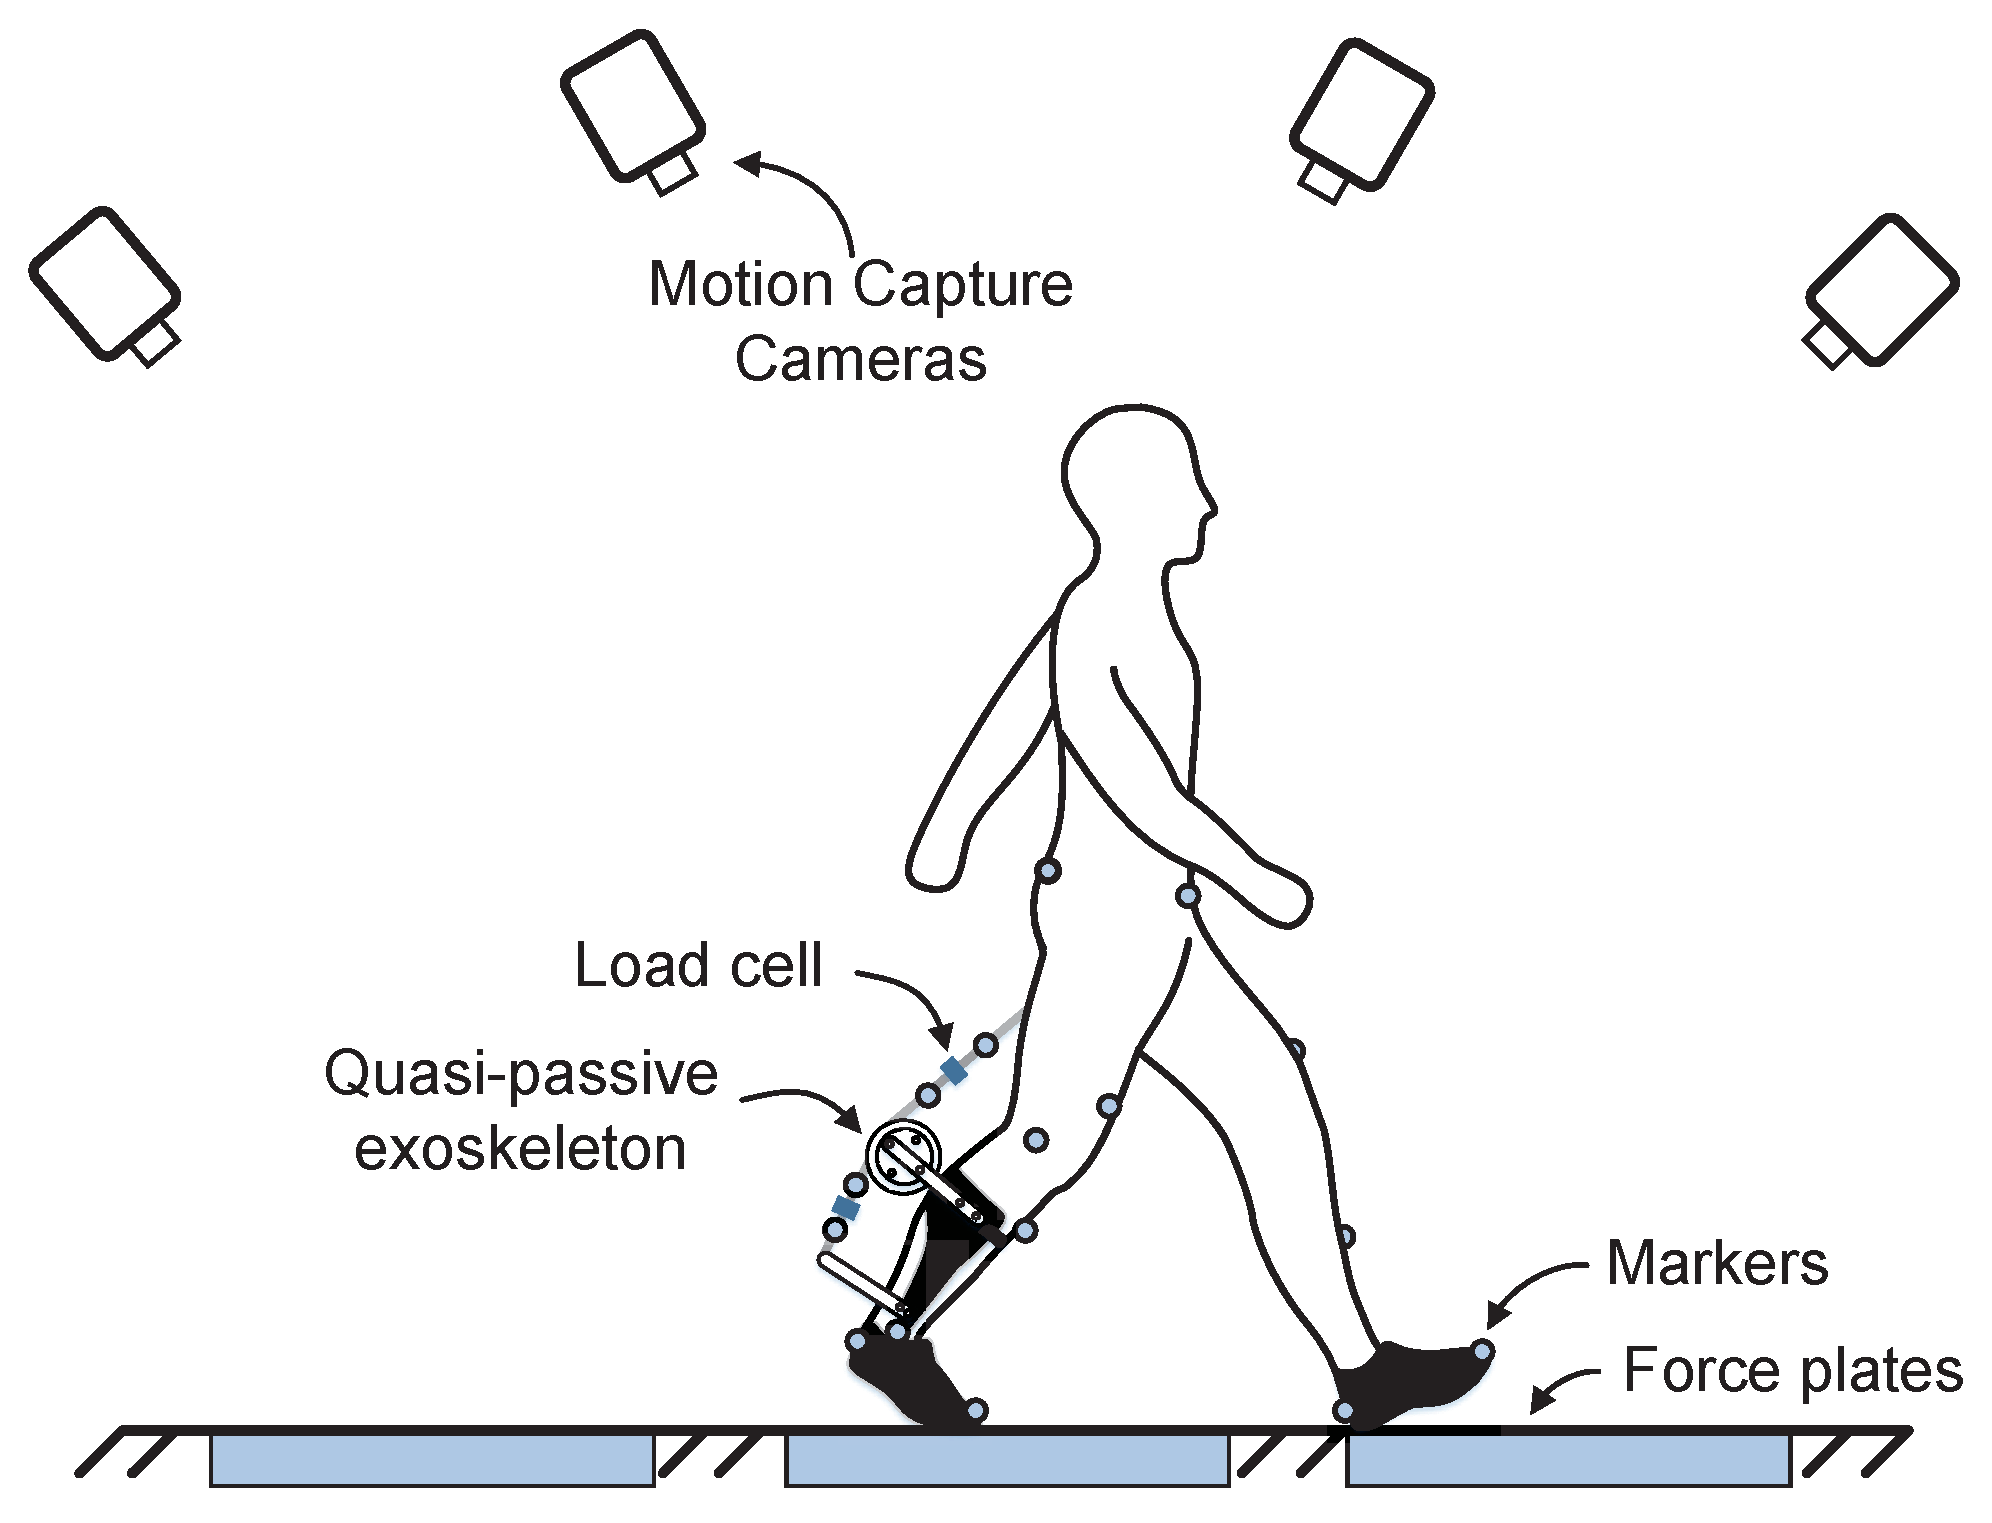
\includegraphics[width=8.5cm]{environment.eps}
	\caption{Experiment setup of exoskeleton evaluation. Experiment environment of ankle power evaluation. Motion capture system (including six  cameras and 15 makers) was used to collect joint kinematics information and three force plates in pathway were used to measure ground reaction forces. In order to calculate the exoskeleton power, two load cells were used to measure the forces in the two ropes. Subjects wore exoskeleton only on their right ride. Markers were placed on lower limbs following the Helen Hayes marker set.}
	\label{fig:Environment}
\end{figure}

The measurement setup is shown in Figure \ref{fig:Environment}. During all trials, the kinematic data of lower limbs were recorded by 15 reflective markers attached on the participates following the Helen-Hayes marker set\cite{RN24}. The markers were tracked by the 3D motion capture system with six cameras (Motion Analysis, Santa Rosa, CA, USA) at a frequency of 120 Hz and analyzed by the Cortex Motion Analysis Software. Simultaneously, the ground reaction forces (GRFs) were sampled at 1200 Hz by three muti-axis forceplates (400$\times$600 mm$^{2}$, Bertc, Columbus, OH, USA), which were embedded in the center of a 12 m long and 1 m wide straight walkway. Trials were recognized as successful only if the subject contacted the forceplates with complete single-foot. For the EXO\_ON condition, to compute the torques and powers generated by the exoskeleton, two load cells (LCM300 Series, Futek, Irvine, CA, USA) were used to measure the forces in the two ropes. Matched analog amplifiers (Futek, Irvine, CA, USA) and a data acquisition module were used to magnify and collect the analog voltage signal of force at 200 Hz. Additionally, two markers were attached on each rope to acquire the direction of the forces applied by the exoskeleton.

In post processing, the marker positions and the GRFs were filtered by a zero-lag Butterworth low-pass filter with the cutoff frequency of 6 Hz and 30 Hz respectively. We obtained joint angles, velocities and accelerations from the marker positions with inverse kinematics calculation in Matlab (MathWorks, Natick, MA, USA). Total joint moments and powers were calculated from the kinematic data and GRFs using Newton-Euler method. 

For the EXO\_ON condition, the total moments and powers consisted of two parts: the exoskeleton part exerted by the exoskeleton and the biological part produced by human joints. The exoskeleton torques were calculated by the product of the force recorded by the load cell and the corresponding lever arms. The lever arms were defined as the distance between the respective force lines and the joint center. Then we obtained the exoskeleton powers by the product of the joint velocities and the exoskeleton torques. Biological joint moment and power produced during the EXO\_ON condition were calculated by subtracting measured exoskeleton torques and powers from total joint moments and powers. To evaluate how much energy is recycled from knee and ankle and finally released to assist push-off, the total exoskeleton work done to the ankle and the knee joints were calculated by integrating the exoskeleton powers over time. For the NO\_EXO and the EXO\_OFF conditions, the biological joint moments and powers were the total joint moments and powers calculated with the inverse dynamics method.

The joint kinematics and kinetics results were segmented into individual strides based on heel-strike events detected from the GRFs. For each subject and each trial, the results in each condition were averaged from heel contact (0\%) to the next heel contact (100\%). All moments and powers were normalized by the subjects’ body mass.

In order to compare the angles, moments and powers of ankle and knee for three walking conditions (EXO\_ON, EXO\_OFF, and NO\_EXO) in a whole stride, one-way repeated measures analyses of variance (ANOVA) was used. To test whether the results are significant or not, we set the significance level of ANOVA at $p<0.05$ for this specific experiment. 

\subsection{Experimental results and discussion}

\begin{figure}[b]
	\centering
	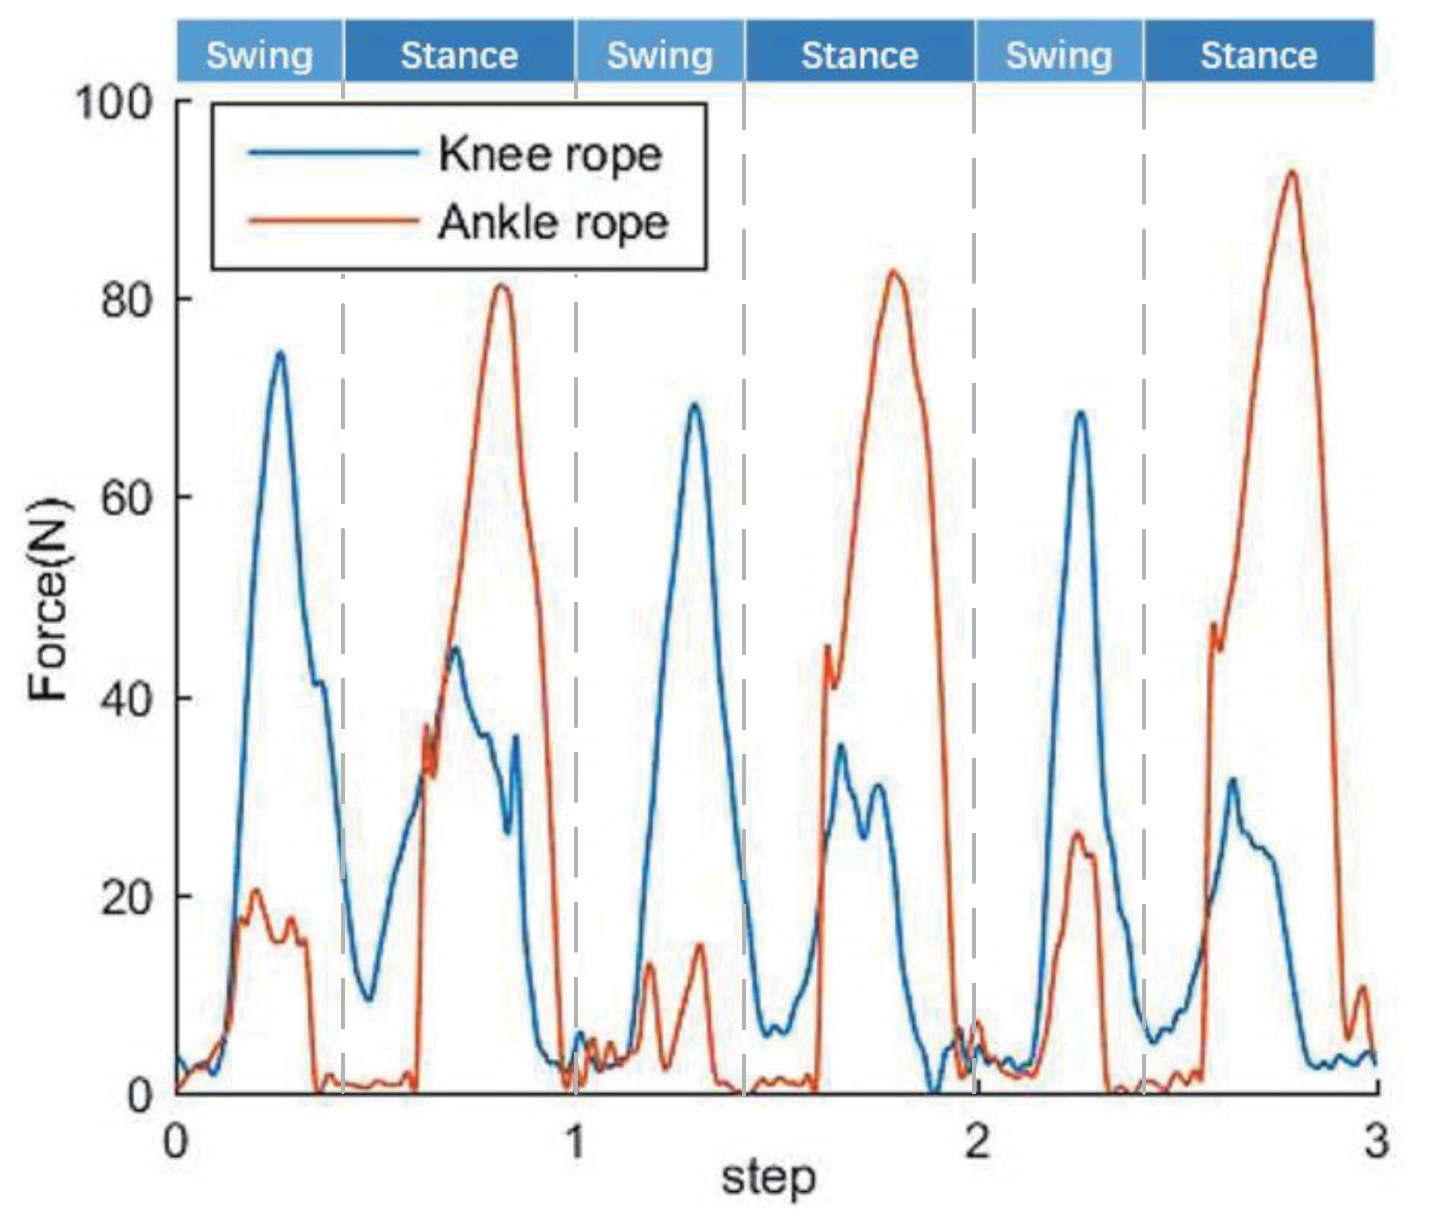
\includegraphics[width=8.5cm]{forces.eps}
	\caption{The forces in the knee rope (blue line) and ankle rope (orange line) in three typical gait cycles.}
	\label{fig:force}
\end{figure}


The functionality of the mechatronics system is verified by the recorded forces in both ropes. The forces in three typical gait cycles of one exoskeleton wearer are depicted in Figure \ref{fig:force}. The average peak force in the knee rope (blue line) in the Figure was 55$\pm$6 N, indicating the spring was stretched to recycle energy from knee extension in late swing. The average peak force in the ankle rope (orange line) was 73$\pm$5 N. It can be clearly seen that the force in the ankle rope can be divided into two stages by different slopes during mid-stance phase. In the first stage, a sharp increase indicates that the already stretched spring began to exert force at the ankle, which led to a sudden change of the force. In the second stage, the slope reduced, indicating the spring was stretched again and began to recycle energy from ankle. \sout{This result demonstrates that the exoskeleton successfully recycled energy from knee and ankle to assist ankle push-off.} \textcolor{red}{This result demonstrates the energy is properly recycled and released by the torsion spring.}

\begin{figure*}[t]
	\centering
	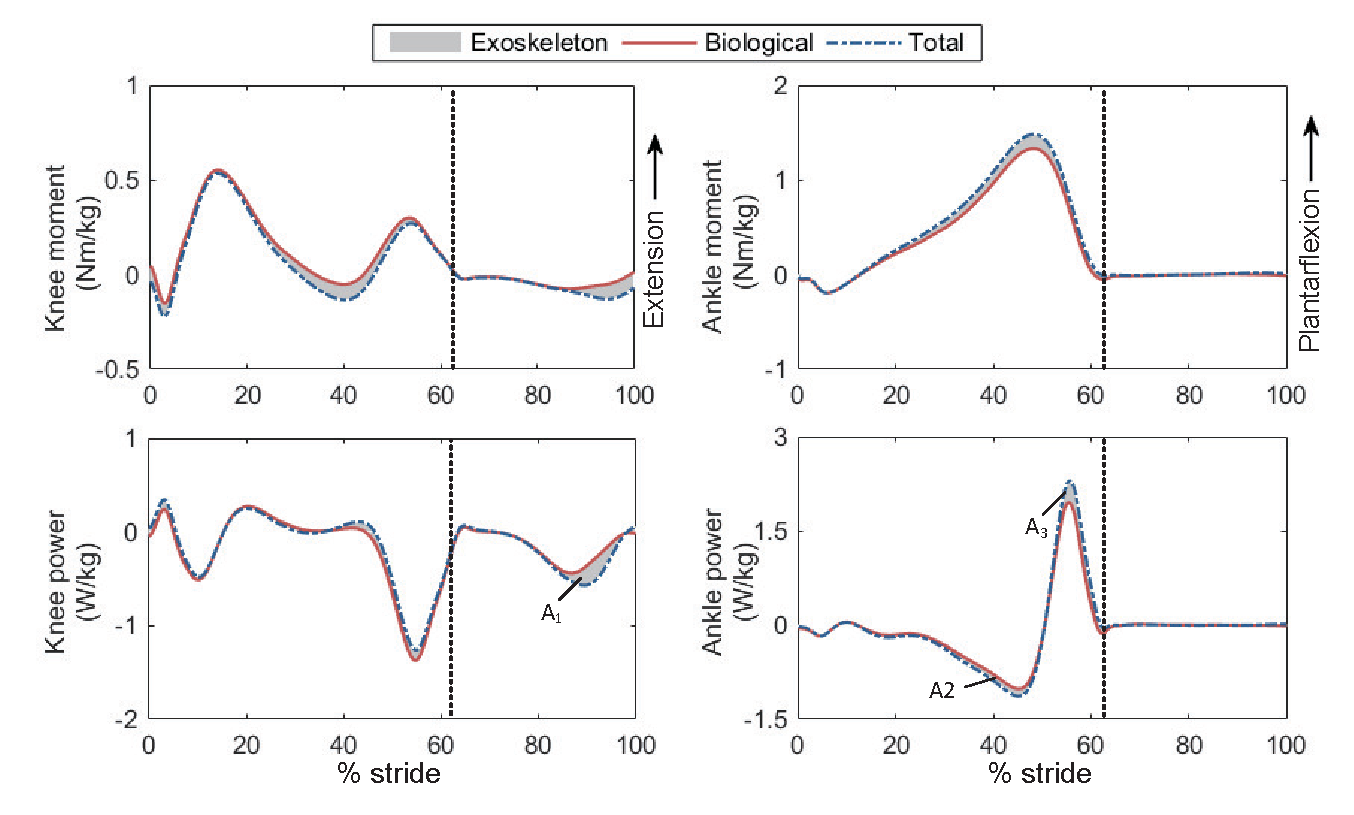
\includegraphics[width=17cm]{exo.eps}
	\caption{The moments and power of knee and ankle joints in the EXO\_ON condition]. The total and biological data are shown with blue and red lines, respectively. The shaded area represents the torque and power provided by the quasi-passive exoskeleton. Data are averaged over all subjects. The stance phase and swing phase are divided by the black dotted line.}
	\label{fig:exo}
\end{figure*}

The total (dashed blue) and biological (red) joint moments and powers averaged over the subjects in the EXO\_ON condition are shown in Figure \ref{fig:exo}. The shaded area represents the torque and power provided by the exoskeleton. The exoskeleton torques were calculated by the product of the force and the corresponding lever arms. 

In the late swing phase, the exoskeleton assisted deceleration of the knee joint. The maximal torque was $0.093\pm0.017$ Nm/kg and the maximal power was $0.271\pm0.037$ W/kg. The total negative work produced by the exoskeleton to the knee joint over 80-100\% stride was $1.43\pm0.36$ J (area A$_{1}$ in Figure \ref{fig:exo}), accounting for 28\% of the total negative knee work during the same period. In the middle and late stance phase, the exoskeleton produced a torque with the same direction as the biological ankle moment. The maximal torque was $0.156\pm0.013$ Nm/kg and the maximal power was $0.449\pm0.029$ W/kg. The minimum power was $0.126\pm0.029$ W/kg. The negative work produced by the exoskeleton to the ankle joint was $1.66\pm0.28$ J (area A$_{2}$ in Figure \ref{fig:exo}), accounting for 13\% of the total negative ankle work during the same period (30\%-50\%). $2.39\pm0.35$ J energy (area A$_{3}$ in Figure \ref{fig:exo}) was finally released from the torque spring to assist ankle plantar flexion, accounting for 20\% of the total positive ankle work (50\%-60\%). \sout{The utilization coefficient of energy of the quasi-passive exoskeleton was about 77.34\%.} \textcolor{red}{The ratio of the energy released at push off to that recycled from the knee and ankle joints was about 77.34\%.}

A part of energy was lost because of the elastic anchor at the pants. The exoskeleton produced an undesirable torque on the knee joint in the stance phase, which also can be observed at the forces in the knee rope in Figure \ref{fig:force}. The maximal torque was $0.083\pm0.024$ Nm/kg and the corresponding maximal power was $0.177\pm0.069$ W/kg. In normal walking, human’s knee joint undergone small flexion in stance, which caused the distance between the anchor on the thigh and the clutch-spring unit decreased. Since the pants were not entirely rigid, there was still some residue force in the rope after the knee clutch locked. As the knee flexed and extended, the residue force exerted a resistive torque at the knee joint and was not passed to the ankle during plantar flexion, which means some energy supposed to be recycled in the torque spring actually was dissipated by the pants. This is an inevitable side-effect for an elastic anchor and might be reduced if a better connection method can be applied. The flexible exoskeleton built by Lee \emph{et al.} \cite{exosuit} presented a unique support frame that withstands vertical loads while maintaining the natural curvature of the wearer's lower body, which could be used in the future work.

\begin{figure*}[th]
	\centering
	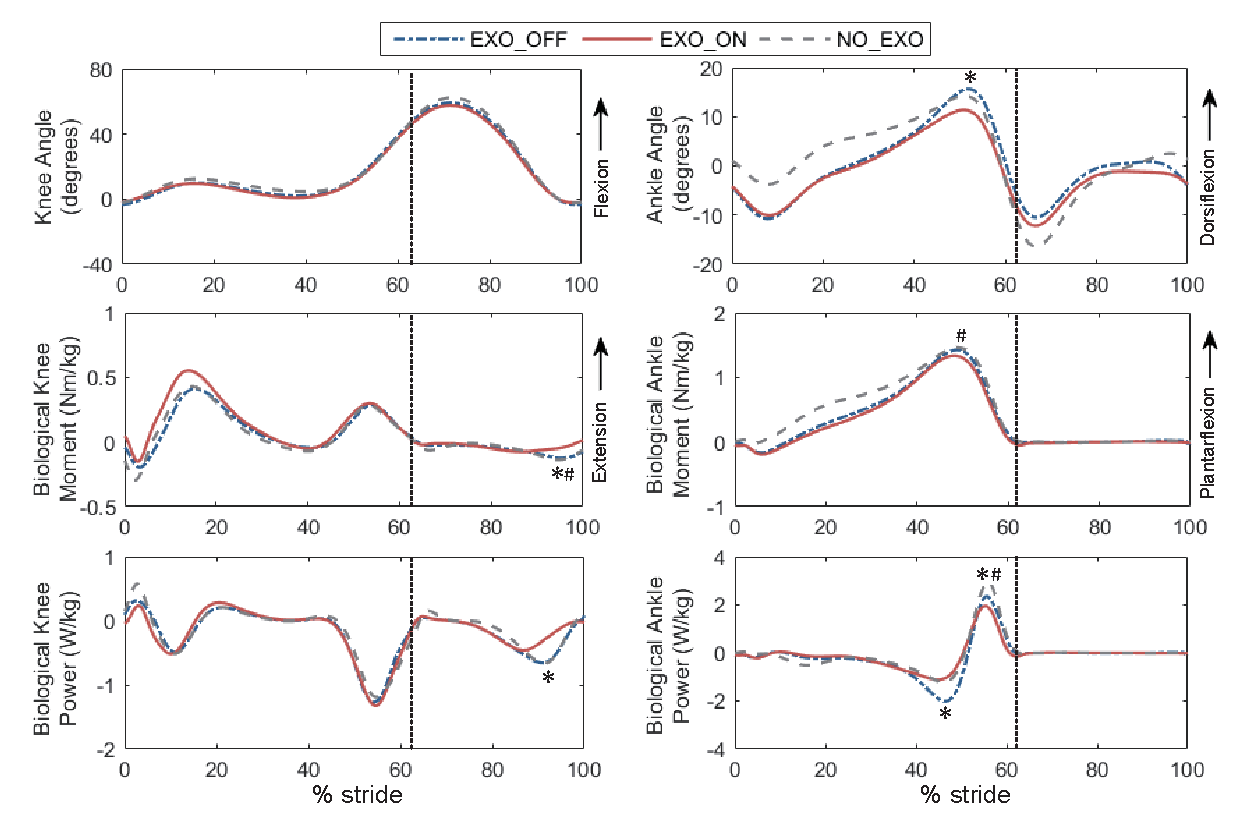
\includegraphics[width=17cm]{compare.eps}
	\caption{Joint kinematics and kinetics results. Comparison of joint angles, moments and powers (top to bottom) for the EXO\_ON condition (red lines), the EXO\_OFF condition (blue dotted dashed line) and the NO\_EXO condition (grey dashed line)across the gait cycle. The stance phase and swing phase are divided by black dotted lines.* and \# indicate significant difference ($p\pm0.05$) when compare the EXO\_ON condition to the EXO\_OFF condition and the NO\_EXO condition, respectively.}
	\label{fig:kinetics}
\end{figure*}

Joint kinematics and kinetics in the three conditions are presented in Figure \ref{fig:kinetics}. The data for the EXO\_ON condition, the EXO\_OFF condition and the NO\_EXO condition are presented by red lines, blue dotted dashed line and grey dashed line, respectively. The knee joint angles over the whole stride for all three walking conditions had no significant differences. The peak ankle dorsiflexion angle during the stance phase of the EXO\_ON condition ($11.6\pm2.5$ degrees) was significantly smaller than that of the EXO\_OFF condition ($15.7\pm3.8$ degrees, $p=0.0298$). The possible reason is that at the beginning of push-off, the exoskeleton output a large torque to assist ankle, which in turn lowered the dorsiflexion angle of the ankle joint to produce the same amount of torque that was needed without assistance. 

The maximal knee flexion moment during the late swing phase was significantly decreased by 43\% and 34.8\% when comparing the EXO\_ON condition ($0.083\pm0.017$ Nm/kg) to the NO\_EXO condition ($p = 0.0004$) and EXO\_OFF condition ($p = 0.0102$), respectively. This reduction indicates that the exoskeleton provided considerable flexion moment and partially replaced muscles on the thigh to generate torque in order to decelerate the shank. In addition, the total biological negative knee power during the late swing phase experienced significant reduction of 15.9\% when comparing EXO\_ON condition ($-0.061\pm0.016$ W/kg) to the EXO\_OFF condition ($p = 0.0138$), which is sufficient to show that the exoskeleton harvested negative power produced by the knee. However, the reduction from the NO\_EXO condition was not significant (p = 0.1875), which might indicate the side-effects introduced by the exoskeleton are still too large and counteracted the assistance.


The most positive effect of the quasi-passive exoskeleton was the reduction of the plantar flexion moment of the ankle joint during the middle and late stance phase. 9.8\% of significant reduction was reported when comparing EXO\_ON condition ($1.347\pm0.096$ Nm/kg) to the NO\_EXO condition ($p = 0.0052$), while the reduction was not significant in terms of the EXO\_OFF condition ($p = 0.0876$). The reductions might reflect reduced calf muscle force due to partial unloading of the Achilles’ tendon by the quasi-passive exoskeleton. The total biological ankle negative work associated with the moment differences was significantly decreased by 31.2\% from the EXO\_OFF condition ($p = 0.0089$) to the EXO\_ON condition ($0.193\pm0.046$ W/kg), while the decrement from the NO\_EXO ($p = 0.4086$) condition to the EXO\_ON condition was not significant. The total biological ankle positive work of EXO\_ON condition decreased by 9.3\% when comparing EXO\_ON condition ($0.119\pm0.025$ W/kg) to the NO\_EXO condition ($p = 0.0027$) and by 29.7\% to the EXO\_OFF condition ($p = 0.0201$). From the calculated data, it can be concluded that the exoskeleton outputs the harvested energy to assist ankle plantar flexion in the late stance. 


\section{Conclusions and future work}
\label{sec:discussion}
In this paper, we presented a quasi-passive lower limb exoskeleton which is able to recycle the energy at the knee joint in late swing extension, and the energy at the ankle joint in stance dorsiflexion to assist push-off. The main functional part of the exoskeleton is the clutch-spring unit which consists of a torque spring as the energy storage element and two active controlled clutches attached at each end of the spring to control the timing of recycling and releasing energy. The novelty of this exoskeleton lies in the energy transferring mechanism from the knee joint to ankle joint, which makes the dissipated energy in decelerating the shank reused to activate the velocity redirection of COM through push-off. Similar to a regenerative braking decelerating a hybrid car, this mechanism has the potential to make exoskeleton more efficient.

The functionality of the exoskeleton is verified by measuring the forces in the two ropes, \textcolor{red}{which indicates the energy is properly recycled and released by the torsion spring controlled through the ratchets.} \sout{The results indicate that the negative work performed by both joints is properly recycled and stored by the exoskeleton, and finally released to assist push-off.} Inverse kinematics and dynamics analysis were performed on eight male subjects in three different walking conditions (NO\_EXO, EXO\_ON and EXO\_OFF). \sout{Except ankle moment in late stance, all of the expected reduction of moment and power at knee and ankle were found to be significant comparing EXO\_ON to EXO\_OFF, suggesting that the strategy of energy recycling and releasing is beneficial to human walking at joint level. However, only during push-off, the power reduction at ankle is significant comparing EXO\_ON with NO\_EXO, indicating the extra weight and motion constraints introduced by the exoskeleton is still nonnegligible in comparison to the benefits.}
\textcolor{red}{Comparing the EXO\_ON to EXO\_OFF scenarios, it can be seen that biological moment and power were significantly reduced during the expected phases of movement (with the exception of the ankle moment in late stance phase). This indicates the strategy of energy recycling and releasing is beneficial to human walking at joint level. However, the extra weight and motion constraints introduced by the exoskeleton have a non-negligible effect on its use. This is indicated by the fact that a significant power reduction in the EXO\_ON case compared with the NO\_EXO case is seen only during pushoff.}

In addition to further testing, we will make some improvements in the mechanical and control aspects. IMUs (Inertial Measurement Units) will be used to acquire the knee angle as an input to the control system \cite{IMU2}. Since the pressure sensors underfoot cannot provide any information in the swing phase, knowledge of knee angle will facilitate a better control on the time to engage the knee clutch, which is now determined by a time delay after toe-off. Also, effort will be made in making the clutch-spring unit lighter and smaller to alleviate the side-effects caused by extra weight as seen in the experiment. Round shaped DC motors will replace the highly integrated rectangular servo motors which makes a lot of spaces and materials wasted in the frame. 

Based on the described work, there are a number of follow-on works that will be addressed in the future. First, lower limb muscle activities and metabolic cost will be measured to evaluate the performance of the exoskeleton at physiological level, which will also provide us with more details about how the exoskeleton interacts with human. 

\begin{acknowledgment}
This work was supported in part by National Natural Science Foundation of China under Grant U1613206 and Grant 61533004, Beijing Municipal Science $\&$ Technology Commission (No Z161100000516033) and Guangdong Innovative and Entrepreneurial Research Team Program under Grant 2016ZT06G587.
\end{acknowledgment}
%%%%%%%%%%%%%%%%%%%%%%%%%%%%%%%%%%%%%%%%%%%%%%%%%%%%%%%%%%%%%%%%%%%%%%

% The bibliography is stored in an external database file
% in the BibTeX format (file_name.bib).  The bibliography is
% created by the following command and it will appear in this
% position in the document. You may, of course, create your
% own bibliography by using thebibliography environment as in
%
% \begin{thebibliography}{12}
% ...
% \bibitem{itemreference} D. E. Knudsen.
% {\em 1966 World Bnus Almanac.}
% {Permafrost Press, Novosibirsk.}
% ...
% \end{thebibliography}

% Here's where you specify the bibliography style file.
% The full file name for the bibliography style file 
% used for an ASME paper is asmems4.bst.
\bibliographystyle{asmems4}

% Here's where you specify the bibliography database file.
% The full file name of the bibliography database for this
% article is asme2e.bib. The name for your database is up
% to you.
%\bibliography{walking}
\bibliography{exoskeleton}

%%%%%%%%%%%%%%%%%%%%%%%%%%%%%%%%%%%%%%%%%%%%%%%%%%%%%%%%%%%%%%%%%%%%%%
\clearpage
\listoffigures
\clearpage
\listoftables
\end{document}
